% !TEX program = xelatex
\documentclass[utf8,oneside]{ctexbook}
\usepackage{amsmath}
\usepackage{hyperref}
\usepackage{graphicx}
\usepackage{ctex}

\title{城市标度律的生成模型}
\author{修格致}
\date{\today}

\begin{document}
\begin{titlepage}
    \maketitle
\end{titlepage}

\chapter*{摘要}

我们生活在一个城市的时代,到21世纪末,大部分人类都将生活在城市之中。我们将集中讲述人类是如何进入城市的,以及进入城市后城市组织将会面临什么样的问题。在这里,研究对象不仅仅是单个城市,亦是城市体系,城市的工商业组成,以及市民在城市中的分布规律。

世界各国在快速城市化过程中,集中涌现出很多有共性的模式与问题。其中包括空气污染、城市热岛现象、能源消耗问题、社会空间不平等以及很多与可持续发展有关的问题。为了向决策者提供可靠的理论和新范式来缓解这些城市问题,对城市结构与演变规律进行建模成为尤为重要的一环。基于简单规则而可解析的统计物理模型可以在不同的角度给出城市发展机制的阐释和预判。近年来,可供城市研究参考的数据越来越多,建模的置信程度也在逐渐提高,这使得此类简洁有力的物理模型能够提供更好的连接理论和经验结果的工具和概念,从而在城市研究发挥重要作用。因此,构建可定量研究、能解释尽量多的城市现象、并有预测性的城市科学是城市研究中极具潜力的发展方向。

本文将总结几类常见的城市地理现象的物理解释。我们关注的问题有城市人口分布、城市分隔模式、与基于位置的城市功能稳定性模型。我们将给出这些模型的描述与内在机理解释。最后我们将给出原创性的一部分工作,关于城市中亚线性与超线性模式的出现与城市功能优化。用简单的物理模型来描述复杂的地理现象,并尽量优美地勾勒地理世界一直是所有科学家的诉求。在大数据时代,我们将面对很多基于数据探索挖掘出的但有待验证的规律,而原理在任何时代都是稀缺的。而自然-人文条件到地理现象因果推断的链条可能可以由统计物理的生成方式复现,这也是我们进行这类研究的初衷。

\tableofcontents

\chapter{绪论}

纵观全球各地与人类文明建立的各个时期,城市的出现与发展是普遍存在的话题。随着城市化与全球化成为一种必然趋势,预计在本世纪末,世界大多数人口都将生活于城市之中\cite{batty2013}。城市形态各异,却通常有着相似的特征:在城市之间,人口、思想、交易和服务产生了城市间多样的交互流;在城市内部,随着空间的集中,个体之间的距离减小,呈现出特定的空间分布与联系;城市多个组分之间相互作用、互依互存的关系构成了复杂的城市生态,允许技能和能源资源的专业化和共享。如帕特里克·葛底斯所言,城市不仅是空间场中的场所,也是时间场中的戏剧。可以认为,城市是人们聚集在一起相互“互动”的地方,是人类社会发展的必然结果。城市中存在着大量组分(如个人、机构和政府)的相互作用,使得我们可以观察到的大规模城市结构在时间和空间上的演变\cite{Barthelemy2019}。例如,在经济学中,城市的优点主要被解释为宏观的规模效应的实现,即因规模增大带来的经济效益提高,而城市体系的大小通常用微观的人口数来衡量。这代表了一种通过特定的微观生成机制来研究宏观指标的思想,微观尺度的简单规则会生成复杂的宏观现象。基于这一思路,我们认为构建简洁的物理模型并结合日益丰富的城市数据,可以帮助我们复现城市中的统计属性,理解城市运行机制。

城市现象是多组分相互作用构成的多尺度的复杂现象。以单个城市为研究对象,若这一城市是它邻域上最发达的区域,有着最先进的生产能力,则它可以从周围吸收生产资料,从而更快地促进邻域的经济和科技流动\cite{Arbesman2009}。然而,如果将视角扩大到较大区域内的城市体系演化,我们会发现城市之间的增长速度是不尽相同的\cite{BerryThe}。以解释人口增加导致城市在空间分布特征变化的一般规律为例,人的空间分布表现出从家庭($\sim 0.01$ km)到洲际($\sim 10000$ km)的各种尺度的聚类。通过对经验数据的研究,科学家总结出针对城市规模分布的简单幂律规律,发现了人口密度波动是规模的函数。即\[n(N) \propto N^{−2}.\]这个函数形式的意义在于,规模越大的城市频率越小,并且随城市的位次是一个幂指数为$-2$的幂律衰减形式。在这里,城市的规模主要指的是人口规模。使用随机场理论和统计物理学的技术,我们证明这些幂定律从根本上来说是人类无标度空间集群的结果,也是人类居住在二维表面上的事实。从这个意义上说,两个空间尺度上尺度不变的对称性与城市社会学密切相关。通过构建物理模型,可复现城市中的统计属性,有助于我们深入理解城市分中心的区位分布与规模分布的耦合关系,对多中心性城市的共同特征和面临的城市病出现的临界条件,同时也对我们理解人地关系和城市扩张所面临的瓶颈有着很多启示作用。从二阶联系角度,曼纽尔·卡斯特尔在1989年将当代城市定义为“流的空间”。场所、空间、与构成它们的活动彼此关联\cite{BerryThe}。对一些综合产业(如电影业)来说,产业的重组与重新聚集,与城市地理中心的模式重建的关联可能会对城市化模式产生重要影响\cite{doi:10.1068/d040305}。人类在不同尺度上的交互使得人类社会在不同层次上呈现出不同的模式。在长期演化过程中,城市尺度逐渐显示出了自己的独特之处。这个尺度是相对固定的,城市内部与城市间的增长规律有显著的区别。在城市间尺度上,经济、人口、基础设施建设等方面的增长速度关于城市规模呈现非线性关系,这导致在大尺度上,城市规模的频率正比于城市排名的一个方幂(Zipf's law);而在城市内部,人与人的交互、政府对有限的城市资源的配置导致城市空间异质性的出现,形成单中心或者多中心结构。供应能力方面,城市可被视为最小的能承担所有必要的个体需求的单位。移动模式方面,城市内的移动是家-工作地的双锚点结构;城市间呈现单锚点结构。

基于以上观测与问题分析,我们认为,城市科学的研究必须从多尺度、多角度进行研究。在尺度方面,城市可以分为人类分布和活动的个体尺度,城市内部活动和交通的城市内尺度,以及大区域范围的城市间尺度。个体尺度的研究问题主要有人类移动性模式、微观尺度的社区结构等问题;城市内尺度的研究对象主要是城市分形等形态研究、城市活动空间、城市交通、动态的城市生长机制等;城市间尺度的研究问题则较为复杂,本文探讨的主要问题是城市间标度律、城市聚集体的形成问题和在不同限制条件下的各种性质的讨论,以及城市的涌现与变迁。在多角度方面,我们考虑城市组织的多元构成,各组分间复杂的相互依存、相互促进关系构成了丰富的开放城市系统。人口统计数据库的可访问性和统计物理工具的应用使这个领域的研究受益匪浅,这些工具使人们能够识别和分析城市形态和标度律特征的普遍性。

从城市间尺度来看,我们关注城市空间特征的统计规律,以及城市逐渐形成、生长、交互、博弈的演化规律。城市发展速度符合一定的统计规律,由此我们可以进一步挖掘城市空间类型与排序特征,并通过基本的物理模型复现城市现象与秩序。城市人口的聚集效应实现了城市生长与形态学研究,现有模型重点关注已有人口和资源聚集而形成城市的过程、以及新的人口和资源如何添加到城市之中的配置规律。从基于传统格点网络,到基于连续空间的点过程,对城市的研究从空间的横向扩展延伸到固定区域限制下纵向的资源累加。城市的发展是长时间尺度下、高度异质性的环境中不断演化发展的过程,城市的涌现、扩展、多中心现象、以及后期的城市收缩,体现了有限资源下的空间配置问题,考虑现实资源限制的城市演化模型进一步揭示错综复杂的城市现象背后的规律及原理。

在城市内部,城市形态反映城市地理环境与发展模式,设施配置分布支撑城市的资源供给,交通实现了动态的交互与生长。城市的形态特征受到局部地理环境、已有人口及社会经济等因素的影响,形成特定的几何与功能特征。城市交通塑造城市形态、联系城市的物质空间,路网演化是长时间尺度上城市结构逐步变迁、优化的体现,它们都是研究城市动态的重要切入点。在城市内研究城市的发展我们将更多地考虑空间与经济资源的限制,这些为传统的生长模型提出了更多的挑战。生长模型本身也在不断引入新的机制,如基于记忆效应的生长模型,预测出更为准确的指标,并且得到更符合实际情况的模拟结果。

城市有限的环境资源使得对城市的分析有了一个抽象的上限,考虑到更为现实的复杂情形,城市不应仅仅被看作一个简单的多组分实体,而是各组分相互依存、相互作用的城市生态系统。在前述内容中我们所描述的城市涌现、迁移、收缩等可以看作复杂的城市元素空间相互作用过程的抽象。我们考虑微观元素的空间交互,城市空间超越网络性质的拓扑特征,并基于空间博弈演化的模型,探讨空间纵深与资源调控下城市这一大型系统的稳定性和可持续发展能力。我们将对空间多主体行为,城市多要素的交互关系及城市生态系统的稳定性条件进行探讨,刻画城市生态系统的复杂性、开放性与变动性。

统计物理学通过构建一个微观模型理解复杂系统,从而得出可以在大规模经验数据上进行检验的分析和预测模型。近些年来,随着城市数据的增多、数据意识的逐渐增强,地理学在传统研究方式之外也增添了很多量化方法,使得我们能够构建量化的城市科学,以识别和建模城市的种种基本现象。特别是,信息和通信技术已经成为实现城市数据采集的重要平台,这些新技术很可能会影响我们对城市空间结构、动态演变的理解,进一步推动有效的理论模型和新的范式来帮助我们认识城市,并缓解一系列关于能源依赖、社会空间不平等、经济发展可持续等的城市问题。

\chapter{城市间尺度:Zipf律、城市聚集体、城市涌现与变迁}

尽管我们很难找到一个城市的通用定义,但城市的优越性是很显然的。在几乎所有的国家,人口都在不断涌入城市。这给城市带来了更快的发展速度。微观增长动态如何塑造区域增长的宏观趋势的固有性质引起了经济学家,城市研究,流行病传播和统计物理学研究的极大兴趣。城市复杂系统的空间异质性和自组织使其能够产生聚集效应\cite{Keuschnigg13759}。城市作为人类栖息地的密集结构,在众多领域发挥着微妙的作用,同时为公民提供有效的生活方式。城市的这种优势吸引人们进入城市地区,这加速了城市科学的发展。城市科学的几个主要问题是道路网络发展,城市扩张以及城市之间的共性和差异性。除了个体层面的动态之外,维度空间上的社区结构也不完全等同于偏好依附等简单机制。例如,在城市内部,个人倾向于靠近,形成现代城市,而他们可以很好地适应某些等级结构,而在空间上保持很远的距离。这些事实表明:城市复杂系统的空间性质解释了不同观测水平的结论差异。城市的空间性是城市的固有属性。

在错综复杂的城市现象中,空间统计学家们抽象出了以标度律、城市分形为代表的一些理解角度,它们可以解释不同尺度上都成立的一些普适规律。另一方面,这些城市规律可以用随机过程的方法得到复现,这些方法也在一定程度上克服了城市发展难以通过实验验证的困境。此类数理模型的大量研究使得我们有理由相信,这些城市规律可以由更微观的机制复现,而且这些方法对于未来的预测都是有意义的。本章将综述不同的城市现象对应的统计物理模型,并给出其中重要的原理阐释。


城市的各种要素所形成的网络枢纽或结点呈现高度的不对称性。这是经济规律的外在表现\cite{BerryThe},其竞争的本性驱动了城市功能,并影响力城市的形态与结构,使得城市格局体现出小者众多、大者甚少的状况。这种尺度问题通常被称为标度律问题(scaling laws)。在城市问题中,标度律往往表现为幂律的特征。即$P(n)\sim n^{-\gamma}$. 在统计意义上,这种幂律特征表明,研究尺度放大的时候,城市问题的结论是自相似的。也可以说,城市问题不存在特征尺度,或者说在不同的尺度上城市问题都是由相同的机制驱动的。在物理上,这类系统的研究有悠久的历史。具有标度律的系统往往处于临界状态,在临界状态的系统的最显著特点是相关长度是无限的。举例来说,铁磁体在达到临街状态时转化为顺磁态,那么该磁体在任意小部分发生自旋方向转化后都会快速影响磁体的所有其他部分。一个活跃的城市系统之中也有着类似的特点。所以我们可以说,幂律行为城市系统的生态性的重要表现。

\section{城市间标度律}

不同属性的网络,以及与之相依的空间和场所,在数值、尺度、形状等方面都有着一种内在的秩序。根据这个性质,我们可以首先探究空间的类型与排序,以得到城市发展的统计规律;进而,我们可以通过一些基本的物理手段,来对这些模型进行复现。

本文中涉及的主要方法都是基于复杂性理论的。复杂性理论将系统看作是自下而上的、由基本成分组成的层级结构,基本成分构成了网络,个体和组团在网络中通过社会和经济活动相互作用,系统的功能则是这些相互作用的表现。即网络交互的指标代表了网络的功能。像城市这样的系统会不断进化,为了实现规模经济,现代社会对集聚的推动力通常会促进城市生长。但同时城市也是自上而下规划的产物。城市不光是在变大,亦是在变得愈加复杂。人们是如何被吸引到城市中来、选择哪一个城市,是一个核心问题。这个问题的答案直接导致了城市之间发展速度的分布规律。这也是城市标度律的一个体现。我们将介绍几个与此相关的模型。并分析它们的直观含义。

我们首先分析一个基础的情形。Krapivsky和Redner在2001年的\cite{PhysRevE.63.066123}中提出了一个生长网络模型(Growing Network, GN)。该模型认为,刨除最初的几个结点,每次网络增加一个新结点的时候都会与已知的一个结点建立连边。选择已知结点的概率正比于已知结点的度(即连边个数)。作者对该模型的分析颇有启示意义。首先考察该过程可以建立的动力学方程
\begin{align} 
    \frac{dN_k}{dt} = \frac{A_{k-1}N_{k-1} - A_k N_k}{A} + \delta_{k,1},\notag
\end{align}其中$A_k=k$。由于每增加一个结点,总的度增加2,这个GN模型可以改写为\begin{align}n_k &= (k-1)n_{k-1}/2 - kn_{k}/2 \text{, for all }k \geq 2, \notag\\
    \Rightarrow n_k &= \frac{k-1}{k+2}n_{k-1}\notag\\ 
    \Rightarrow n_k &= \frac{6}{(k+2)(k+1)k}\cdot n_1\notag\\ 
    \Rightarrow n_k &\sim k^{-3}.
\end{align}这样我们就推导出了GN模型下的幂律分布。论文中的模型就到此为止了,但是我们发现,其中有一些值得注意的点可以探究。该模型的意义是新迁入的人口在某城市“扎根”,是由于他认识了某一个城市的原住民。我们可以进一步假设,他加入网络认识两个、三个、或者更多人的情形。通过相应地改写动力学方程,我们可以得到\begin{align}
    n_k = \frac{k-1}{k+2m}n_{k-1}\sim\frac{1}{C_{2m+k}^{k-1}}n_1\sim k^{-(2m+1)} \label{degm}
\end{align}即如果一个人进入社会的时候,与更多人建立联系,则每个个体的度分布会更加偏态。这是一个很有启示意义的想法。即社会上的弱者不会因为新投入资源的增多而享受到更多公平。因为这种投入也降低了社会上强者不继续补强的概率。所以从人际资源的角度来说,新进入城市的人口随机地加入某一个特定人群,而不是多个社区,是最有利于社会公平的。

另一方面,该文章用到的几个工具也是最重要的处理手段。这几种手段在\cite{Bagrow_2008}中得到了更详尽的分析。该论文详细给出了生长模型的一般处理方法。并讨论了截断效应对模型的影响。我们根据该文章的思路展开一下对增长模型分析工具的一些讨论。

首先是率方程(rate equation)。率方程描述的是一个个体所拥有的平均财富的演化规律。率方程是我们处理个体变迁的重要工具。这个概念来自于化学反应。化学反应的速率与各种离子的浓度有关,率方程描述的就是这个关系。在社会结构中,弹性\cite{gao2016universal}是普遍存在的。一个很有害的群体可以被稀释在一个巨大的城市体系之中。而它增长到足够大的时候,又会对整个社会产生超线性的重大影响\cite{schlapfer2014scaling}。这是因为人群交互量是随着城市规模的增加而超线性增长的。
\begin{figure}
    \centering
    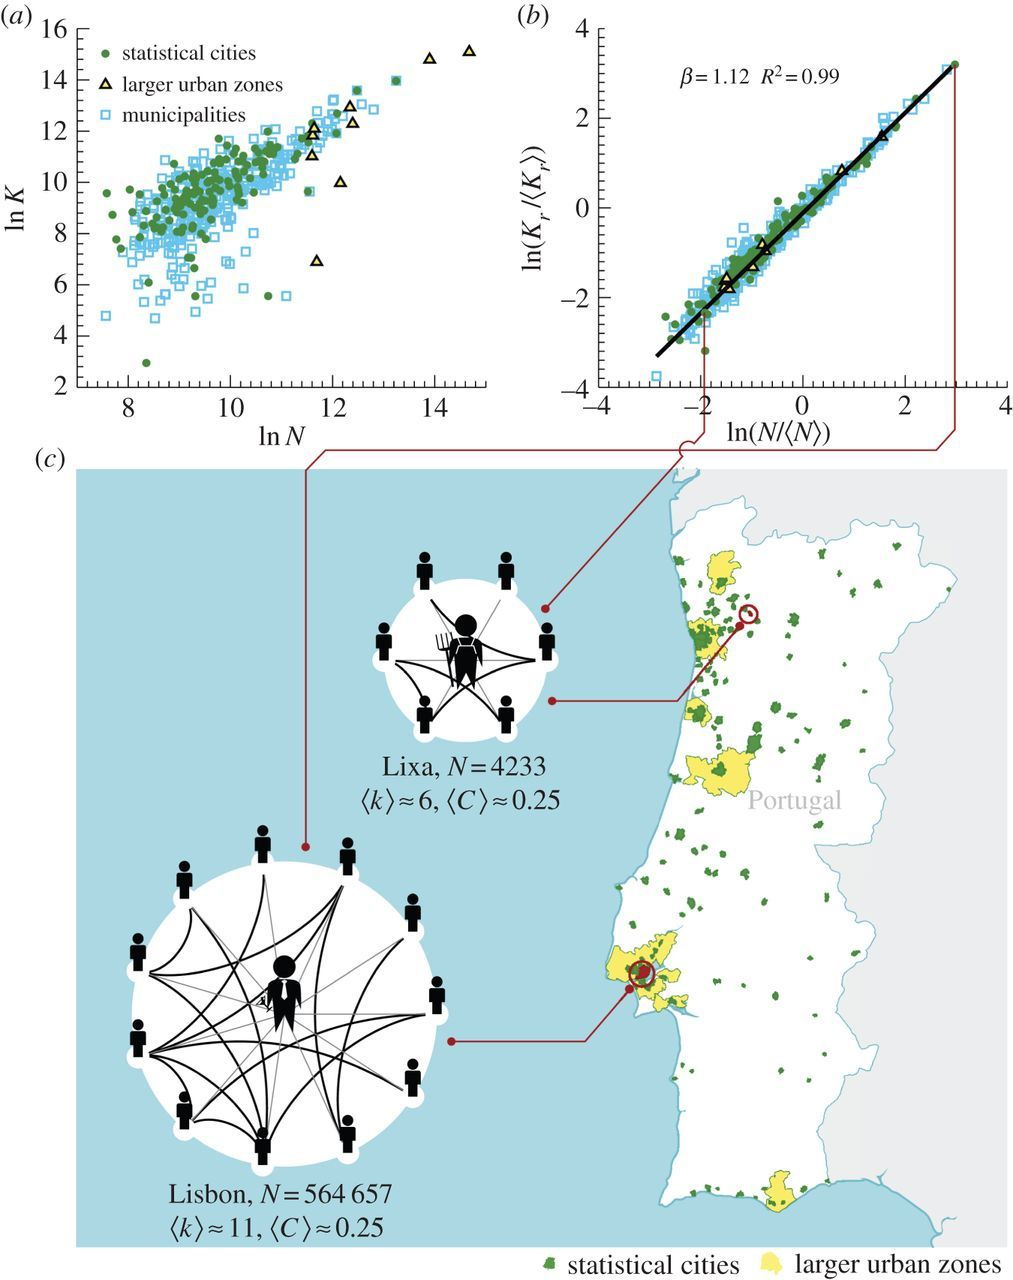
\includegraphics[width = \linewidth]{pictures/rsif20130789f01.jpg}
    \caption{出自\cite{schlapfer2014scaling},人群交互随着城市规模是一个超线性的关系。}
\end{figure}

其次是主方程(master equation)。主方程描述的是群体中拥有度为$k$的点所占的比例随时间的变化规律。是一个群体角度衡量城市贫富变化规律的工具。在随机数学中,主方程可以用来描述群落中种群数量的变化规律。由此可见,有一大类问题可以由同样的数理机制解释。我们可以通过对比物理现象中的数量变化过程与经济地理变化规律来扩展更多的结论。对于空间问题,物理中常见的理解方式是通过场论。已经有学者在工作中用到了场论来处理人类移动性在城市内尺度的表现\cite{molas2017field}。该模型提出城市是一个有单中心的实体。这样的实体中人群移动实际上是一个随机梯度下降的过程。即各个空间位置的关系是动态平衡的。在接下来的研究中,我们也会引入随机斩杀模型的Feynman-Kac公式\cite{PhysRevE.98.052114}来进一步解释移动性过程中的交互问题。主方程推导出的场模型另外一个出路,则是利用电场中的性质,结合生态系统理论,来预测城市群的经济关联关系。如果将每个城市考虑为一个电网中的支路,那么\cite{doyle1984random,Volchenkov2011Random}显示,我们可以通过电路分析中的一些算法来求解城市间物质流动的稳态关系。进一步,我们还将在后面根据此算法来讨论更进一步的城市间物质流动的稳态性质。

在空间问题中,异质性是广泛存在的。GN模型中注意到,在研究随机图的矩时,保证低阶矩的稳定的同时增高高阶矩是一个得到网络异速增长的有效办法。这里我可以总结为,空间异质性的形成是由局部升矩过程导致的。我们在研究了其他一类模型之后,发现其他模型得到了同样的构造方式。根据此,我们也提出了自己的新模型来构造这个过程。我们首先在下面一节中介绍几种城市聚集体模型和其中的升矩关系。再在下面一节的后半部分介绍我提出的一种升矩模型。

\section{城市聚集体的模型与偶发事件}

城市形成的物理理论可以分为两个大类:已有人口和资源如何重新聚集继而形成城市;新人口和资源如何增添到已有的城市之中。\cite{PhysRevLett.79.523,PhysRevE.58.295,PhysRevLett.112.240601}提出的模型解释了第一种情况。直接对第二种机制形成城市建模的研究工作比较少。张江\cite{ZhangScaling,LiSimple}的匹配增长模型提供了类似的思路。笔者在近期的一个工作的一部分即是用两条规则来建立城市间人口分布规律。

第一类模型的思想源于数学上的晶格动力学模型。在二维空间格点上每一个格子有相同的初始人口。随着时间的流逝,人口依照某种半随机的方式进行变化。最终停留在我们熟悉的规律上。这种演化方式通常是升矩的。比如Manrubia, Susanna C.团队在1998年的两篇工作\cite{PhysRevE.58.295, PhysRevLett.79.523}继承了Zeldovich在随机网络的工作,并引领了这个机制在城市科学的相关研究。在人口系统中,地理相关性通常被称为相关场,作为局部人口迁移的动力学机制解释。在总人口为确定值的二维方形格网区域内,记录每一个时刻$t$的每个格点$x$上的人口为$n(x,t)$. 则下一个时刻的人口分布符合\begin{align}
    n(x,t') = \begin{cases}
        (1-q)n(x,t)/p , \text{概率为 } p\notag\\
        qn(x,t)/(1-p) , \text{概率为 } 1-p
    \end{cases}
\end{align}这种机制保证了总人口的恒定,同时(由于均值不等式的成立)增加人口分布的矩$\mu_k(t) = \sum_k n(x,t)^k$. 它的实际意义是不断增加的空间异质性。由于总人口的恒定,该模型可以解释为一个人口迁移模型,即人口不断从乡村区域迁移到城市,迁移到不同城市的速率正比于城市的规模。为了使这个机制得以实现,我们还需要假设对于每一个位置,迁出的人口是该处人口数的一个固定比例$\alpha$。
\begin{figure}
    \centering
    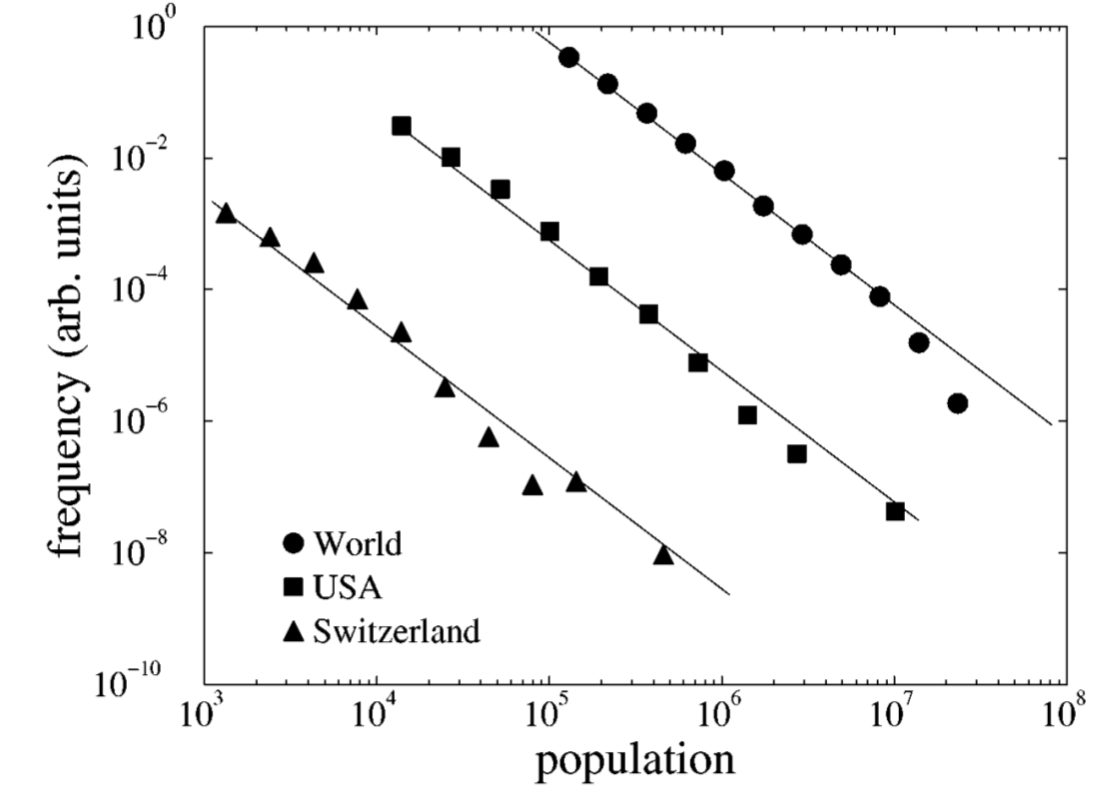
\includegraphics[width = 0.3\linewidth]{pictures/roiiudreal.png}
    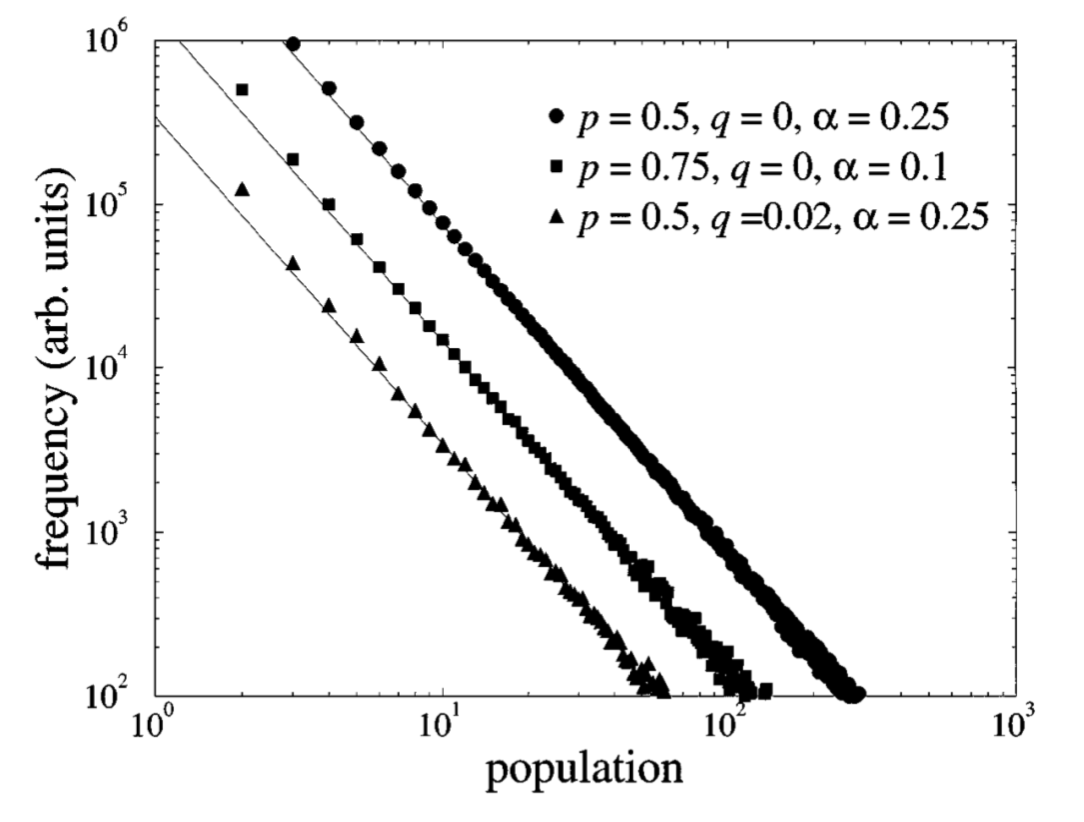
\includegraphics[width = 0.3\linewidth]{pictures/roiiud.png}
    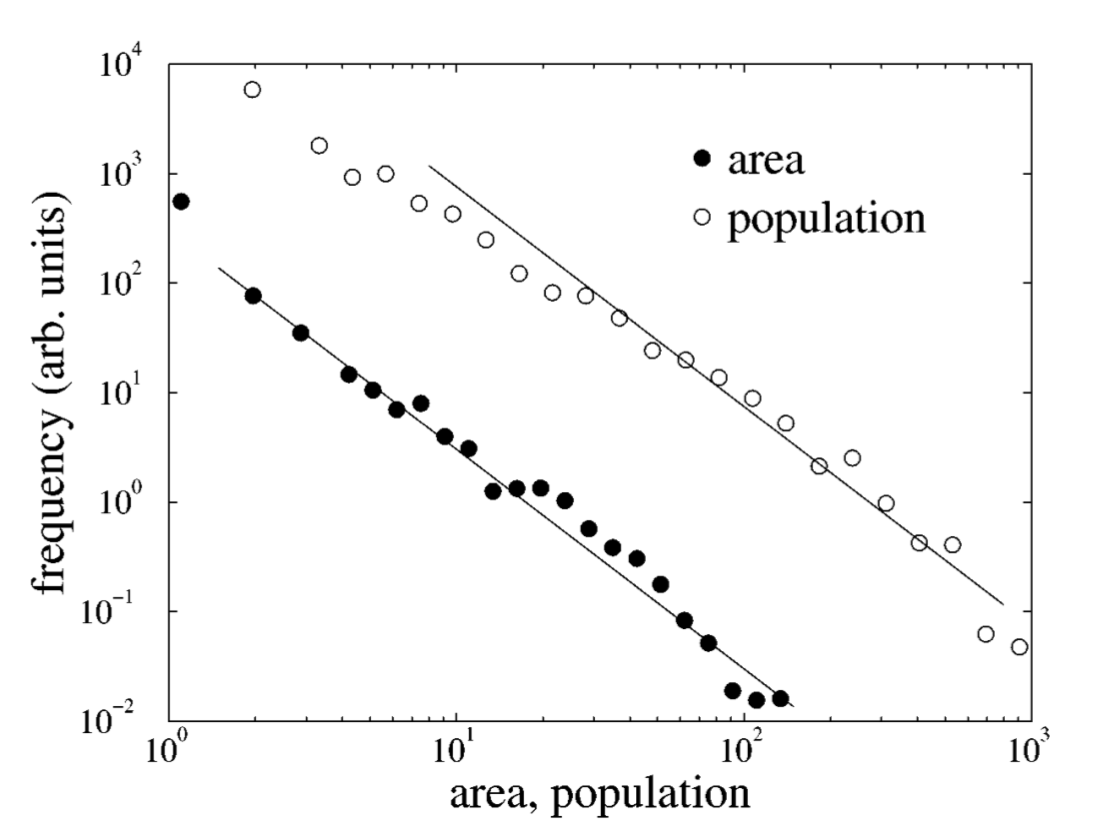
\includegraphics[width = 0.3\linewidth]{pictures/roiiudarea.png}
    \caption{左图:全球2700个最大城市,美国的2400个最大城市和瑞士的1300个最大的自治市的人口分布\cite{PhysRevLett.79.523}. 图中斜率为$-2$ 右图是该文中对于不同的参数的三组模拟结果。我们发现,该模型下不同参数导出的城市人口分布都服从一个参数为$2$的幂律分布。}
\end{figure}该模型可以导出的另一个结果是城市面积的频率。通过假设人口密度高于总人口密度的区域为城市区域,连通的城市区域可以进行面积的统计。城市人口的聚集效应导致城市面积趋近于稳定大小。边际区域上面得到的补充人口与扩散人口数维持动态平衡。

Hernan A. Makse, Shlomo Havlin,H. Eugene Stanley在1995年的文章\cite{Makse1995}中提出的模型更进一步可以解决空间标度律和形态学问题。它符合了两种真实的城市性质。首先,单中心城市的人口密度随着到城市中心的距离是指数衰减的,即\[\rho(r)=\rho_0 e^{-\lambda r}\]其中$\lambda$是密度梯度。其次,在真实的城市中,发展单元在空间上并不是随机分布的,而是以街区的形式规则排列的。而且发展得好的区域的邻近区域通常也是发展得好的。在地理上,这被解释为空间自相关性。基于这两个假设,作者提出了一个相关渗流模型。一个距离城市中心距离为$r$的景观以概率为$u(r)$被占据。这个概率是基于幂律分布的。该模型生成的城市形态具有明显的分形和随机性特征。模型生成的连通集团可以定义为模型生成的城市边界。大型的城市的吸引力使得郊区城市分中心的边界不及中心城市区紧致(compact)。这与如柏林、巴黎和伦敦等城市的真实情况是相符合的\cite{Batty2006}。笔者的模型中利用了一种新的机制来重现这种性质。即不同城市的扩张是独立的,而大城市在城市边缘的人口密度小于小城市的人口密度。从而在土地竞争中占更劣势,使得小城市的边缘更加突出,从而体现出去紧致化的特征。

该模型其他的性质包括城市面积随着相关距离衰减规律。对于不同的衰减指数,连通面积的频率的衰减规律都是一个指数为$2.09$到$2.45$的幂律分布。
\begin{figure}
    \centering
    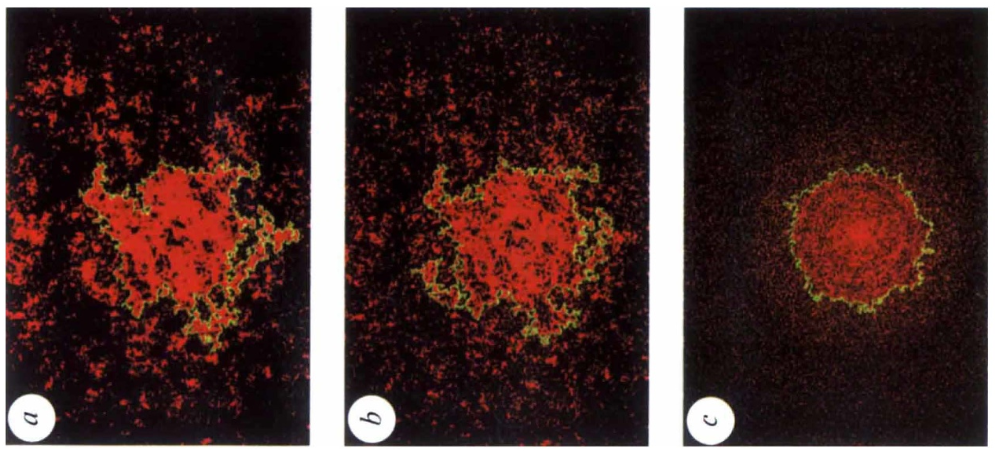
\includegraphics[width = 0.65\textwidth]{pictures/modellingurbanpattern.png}
    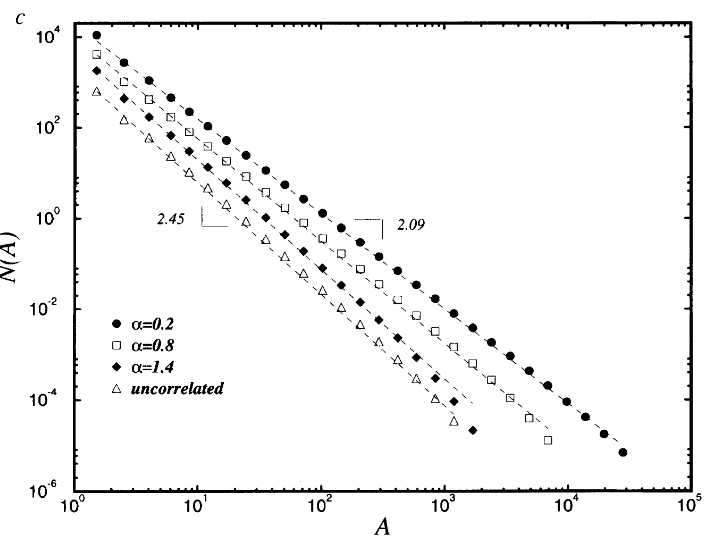
\includegraphics[width = 0.45\textwidth]{pictures/area_scaling.png}
    \caption{上方是\cite{Makse1995}中的模拟结果。前两图分别为幂律指数为$0.6$和$0.4$的情形。可以看出,随着幂律指数的升高,城市的“斑图化”更加明显。城市郊区形成副中心的概率更高。最后一张图表示完全随机的情形,即不同景观之间的发展完全不互相影响。下方是\cite{Makse1995}模型导出的城市面积分布规律。在这里我们认为一个连通的组团是同一个城市。}
\end{figure}

Diego Rybski等人在\cite{PhysRevE.87.042114}中提出的模型是上述观点的扩展。该模型基于的假设是:增长更可能发生在居住空间附近。这个效应由一个距离衰减系数控制。具体实现是每次对所有位置遍历,如果它收到的来自于其他区域的总放射量大于某个阈值,那么这个位置就会被标记为城市区域。这个过程也可以迭代的进行。该模型模拟出的城市面积分布与真实情形在统计意义上是相似的,都是幂指数为$2.5$的幂律分布。

值得注意的是,该模型是一个基于距离衰减的长程模型。该模型更显著的特征是对于位置间的关联通过距离加权,进而得到局部的发展潜力。我们认为这种模型是与重力模型有很大关系的。尽管人口引力一词在国民经济学领域是Stewart于\cite{10.2307/2785468}提出的,但在经济地理研究中,引力模型已经研究了数十年。 Carrothers\cite{carrothers1956historical}对重力和人类互动的潜在关系进行了综述。销售行业的瑞利引力定律描述了相同吸引力的边界范围\cite{reilly1931law}。它依赖着销售业和城市居民的同质性假设。Huff的购物者吸引力定律\cite{10.2307/3144521}提供了代理商在给定地点前往特定设施的可能性。重力模型则可以用来做国家之间的贸易量的建模。它的局限性是在流动和迁移问题建模时,无法反映非对称的情形。有工作将重力模型修正为\[G_{ij} = \frac{m_i^am_j^b}{d_{ij}^c}\]用以回应不对称的情形。但该模型需拟合的参数过多,降低了模型的解释性。可见重力模型在地学和经济学问题中扮演了举足轻重的地位。空间占领背景下的重力模型是比较容易被忽略的,因为被占领的空间的质量只是$1$,从而没有重力模型下强异质性场的问题。\cite{PhysRevE.87.042114}中的模型建立在$N\times N$栅格空间上每两个栅格之间的作用强度由下式定义:\[q_j = C\frac{\sum_{k\ne j}w_k d_{ij}^{-\gamma}}{d_{ij}^{-\gamma}}\]可以看出这个模型的权重项跟Huff模型的吸引力是一样的,并且其中的衰减系数$\gamma$的增大会使得距离衰减更快,进而增加模型的集聚效应。每一个时刻,每个栅格都会评估一下其余栅格对其的总作用。如此迭代下去,会形成一些染色图案。\begin{figure}
    \centering
    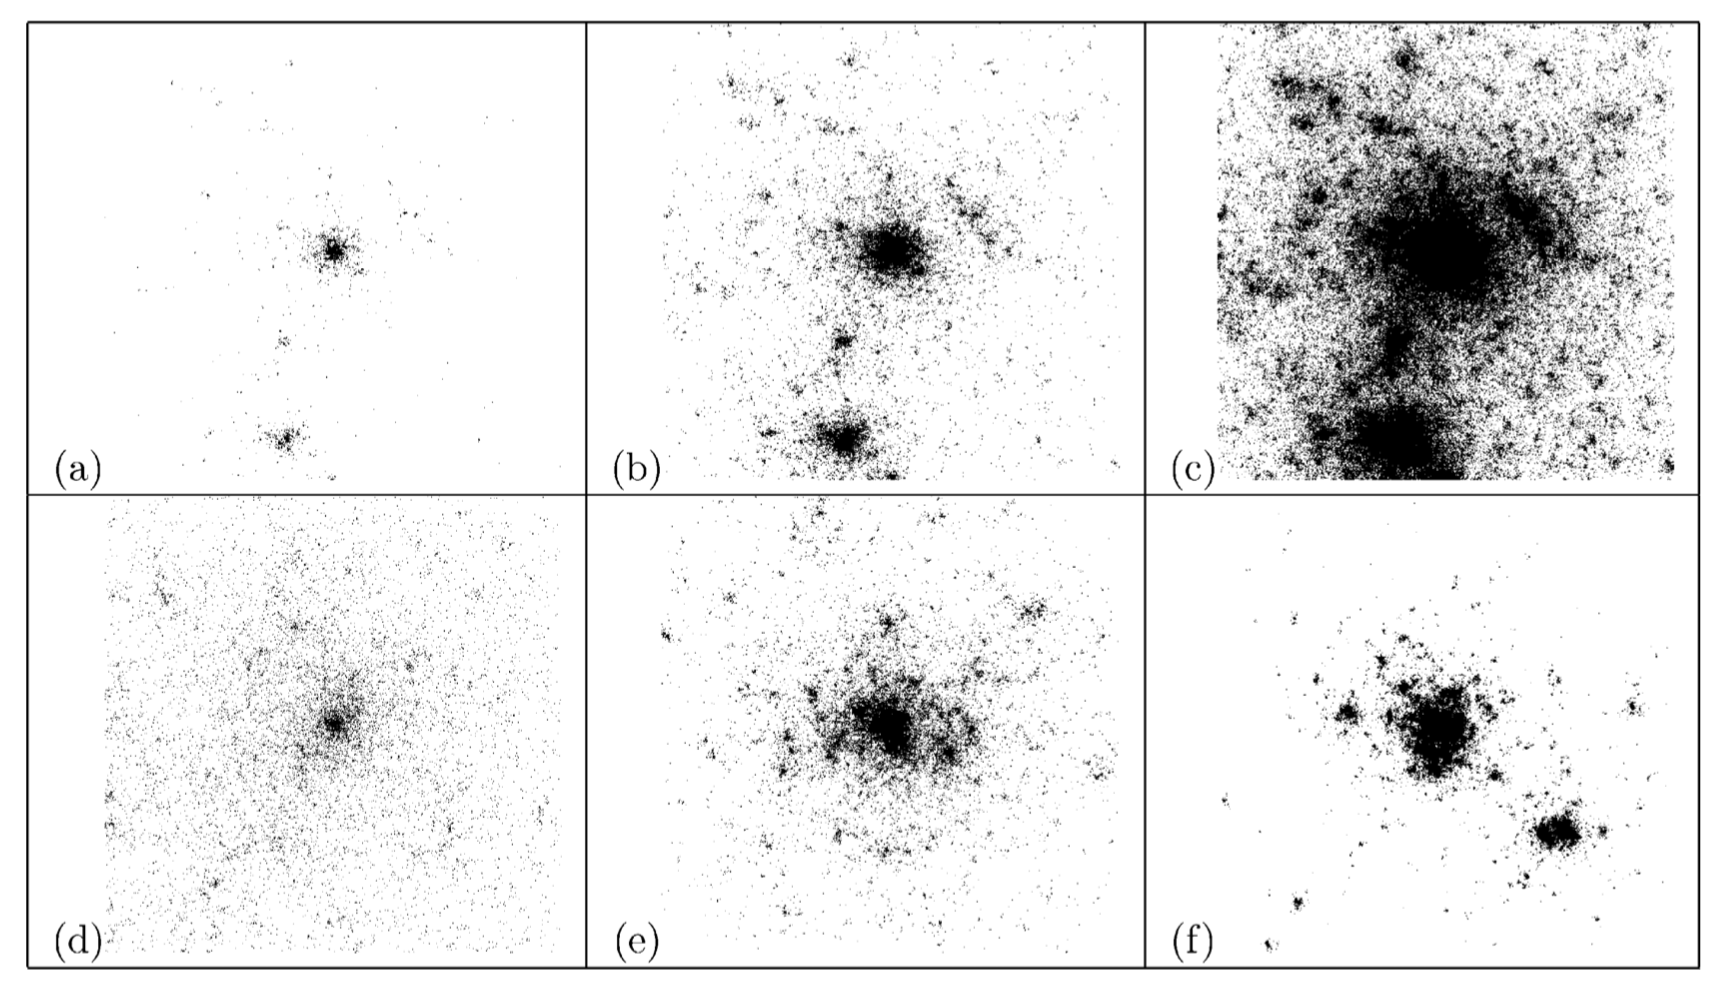
\includegraphics[width=\textwidth]{pictures/distance-weighted.png}
    \caption{前三个图是模型迭代6,10,14次的图案;后三个图是距离衰减指数为2.0, 2.5, 3.0时的城市分布。}
\end{figure}
该模型导出的统计结果可以概括为三条:城市面积的幂律分布、城市边界的分形、以及区域连通性的渗流相变。

基于此类模型,笔者总结了较为一般的模型规律。即反应-扩散模型(reaction-diffusion models)导出空间异质性的基本原理。这一模型假设在城市形成的过程中地理位置上相邻的区域具有高的交互强度(reaction),而相邻区域的人口分布差异促进了人口流动(diffusion),差异越大,人口分布的变化趋势越明显。动力学的升矩过程描述了差异增大的过程,可作为空间异质性增强的合理假设。在$N\times N$的二维格点空间中,给定各个格子分布1单位人口为初始状态。模拟城市生成的迭代规则基于反应与扩散机制——在内部($N-2$)$\times$($N-2$)的格点中以某一指定的顺序遍历格点,通过比较目标格点与其八邻域人口均值($n_{neighbor}$)的相对大小更新格点人口数目,模拟人口迁入($\geq n_{neighbor}$)或迁出(\textless$n_{neighbor}$)过程。具体来讲,假设人口迁出比例为固定的$\alpha$,则目标区域的更新规则为:

\begin{equation}
n(x,t) 
\begin{cases}
	<\overline{n(\delta x,t)}: & n(x,t)=(1-\alpha)n(x,t) \notag\\
	 & n(\delta x,t) += \frac{\alpha}{8}n(x,t)\notag\\
	\geq\overline{n(\delta x,t)}: & no\ change
\end{cases}
\end{equation}
其中,$x$为目标格点,$\delta x$为其八邻域,$\overline{n(\delta x,t)}$为八邻域格点内的人口均值。人口数越多,区域的吸引力越强,就会有更多的人口迁入。在此模型中,更新只在目标格点人口低于邻域均值时进行。我们不考虑人口数值外的其它区域环境差异因素,因此低值格点会均匀地向其八邻域迁出$\frac{\alpha}{8}$比例的现有人口。

这一基于反应-扩散机制的城市生成模型,根据人口分布特征与基本的交互规则模拟城市生成过程,由均匀到聚集分布的升矩机制可以从动力学角度对空间异质性的产生原理进行解释。由此可进一步探讨城市区域性差异及形态学问题:目标格网的选取顺序对人口更新过程及城市格局形成的影响,如随机选取,横向遍历,由中心向四周遍历等;模拟的人口频数分布与Clark定律的吻合程度可对模型进行验证;通过格点人口数阈值(如格点数值小于1)可提取城市范围及平均半径,进而对城市面积量化与形态学研究提供参考。

% 还有Potts models

\section{考虑人口密度的空间生长模型}

我们可以看出传统的格点网络框架将城市发展的范围作为最重点的研究对象。这对传统的城市扩散有着比较好的效果。但是随着城市的发展,越来越多的城市都会集中在相对固定的区域上面。在每个城市内部,高楼的数量则会越来越多,更多的城市资源会向城市中心集中\cite{BerryThe}。这时,我们再用格点模型和斑图动力学来研究空间问题就没有那么合适了。这些模型只能研究空间问题的一些很片面的方面。我们需要考虑空间上小地块上的密度。所以基于连续空间上的点过程就变得尤为重要。

我们先考察匹配增长模型\cite{zhang2015scaling}。该模型的过程是这样的:给定一个有界\(d\)维欧式空间\(S=|x_1|,\cdots,|x_d|\leq \frac{L}{2}.\) \(t=0\)时在原点插入一个结点。结点生成的机制为:每个时刻\(t\),以均匀分布在\(S\)中放置一个新结点\(P_t\),记它的坐标为\(x_t.\) 如果存在一个已有结点\(P_q,q\in\{1,2,\cdots,t-1\}\),跟这个新生成的结点很接近,使得\(||x_p-x_q||< r\),则新结点\(P_t\)存活。否则\(P_t\)死亡。连边机制为:将新加入结点与其\(r-\)临域的所有结点相连。重复这个过程,直到存活的结点达到\(N\)个。这个几何网络会加速增长。因为新加入的结点可生存的区域的测度(为所有存活结点的\(r-\)临域的开覆盖)会越来越大。
\begin{figure}
    \centering
    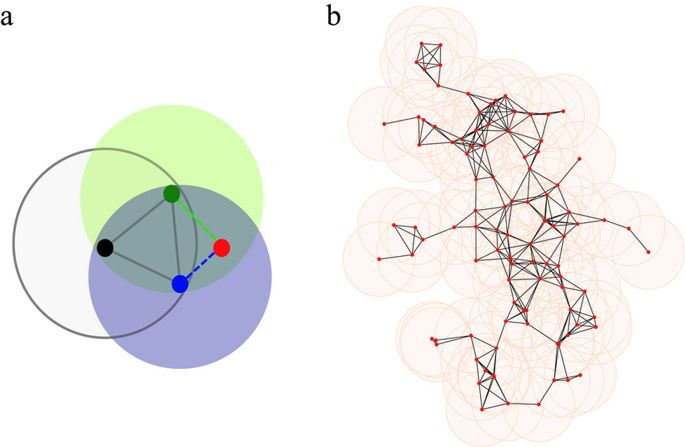
\includegraphics[width = 0.48\textwidth]{pictures/srep09767-f1.jpg}
    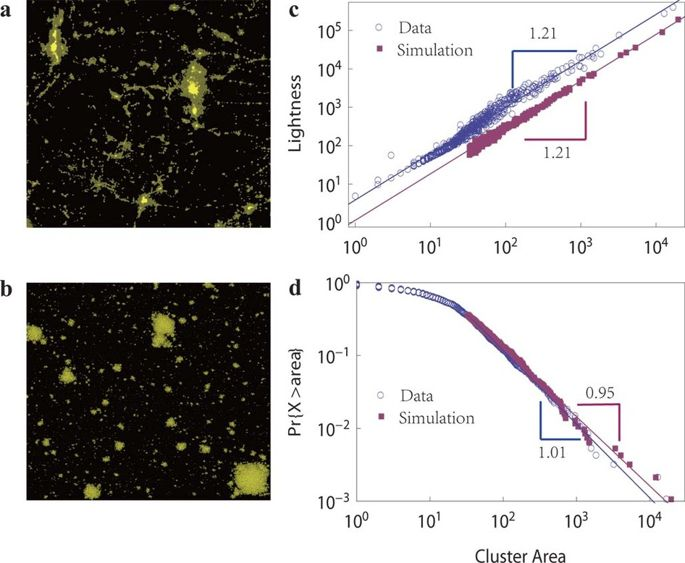
\includegraphics[width = 0.48\textwidth]{pictures/srep09767-f3.jpg}
\end{figure}

这个模型在一定程度上是可以解析的。由于模型的各项同性,在取热力学极限($L,t\rightarrow\infty$)的情况下,这个空间网络会渐近形成一个$d$维球。于是模型给出的第一个性质,也就是这种机制下网络空间的半径$R(t)$是正比于时间的。半径\(R(t)\)(定义为\(\max\{||P_0-P_i||,i=1,2,\cdots t\}\))。以1维正半轴为例,新结点\(P(t+1)\)落在\([0,R(t)+r)\)可以生存,落在\([R(t)-r,R(t)+r]\)可以使得\(R(t+1)> R(t).\)于是增加半径的量的期望为(在\(R(t)\)远大于\(r\)的前提下)
\begin{align}
  &\int_0^Ldx\ P(x_{t+1}=x)\Delta R_{x,t}\notag\\
  =& \frac{2r}{L/2}\int_{R(t)-r}^{R(t)+r} dx\ \frac{1}{2r} (x+r-R(t))\notag\\
  =& \frac{2}{L} \{(2r\cdot [r-R(t)]) +\frac{1}{2}[(R(t)+r)^2-(R(t-r))^2] \}\notag\\
  =& \frac{2}{L} 2r^2\notag\\
  =&r^2/L\notag\\\
  \equiv& C 
\end{align}
所以网络的半径\(R(t)\)匀速增长。所以\(R(t)\sim t\)。对于多维情形,在每个维度上的半径\(R_1,\ldots,R_d\)的增长速率都相同,所以它们的线性组合的增长速率相同。即向任何一个方向的增长速率相同。

第二个问题则是点密度问题。距中心距离为\(\rho\)时,密度\(\mu(\rho,\Theta ,t)\sim \frac{R(t)-\rho}{L^d}\),\(\mu(\rho,t) \sim \frac{(R(t)-\rho)\rho^{d-1}}{L^d}. \)到中心距离在\(\rho\)以内的结点个数\(\sim \rho^d\)。利用这个关系,我们还可以得到存活下来的结点总数以及边数。总人口为:\begin{align}
    N(t)&=\int_0^{R(t)}\mu(\rho,t)d\rho\notag\\
    &\sim R(t)^{d-1}\notag\\
    &\sim t^{d-1}
    \end{align}边数为边数\(v(\rho,\Theta,t)\sim u(\rho,\Theta,t)^2\)(局部每两个边都相连),所以总边数可以写为\begin{align}
        E(t) &=\int v(\rho,\Theta,t)d\sigma\notag\\
&\sim \int t^2\cdot t^{d-1} dt(\text{极坐标变换})\notag\\
& =t^{d+1}.
    \end{align}所以我们有$E(t)\sim N(t)^{\frac{d+2}{d+1}}$。这个结果与\cite{PhysRevX.4.011008}的结果是类似的。这说明局部全连接形成的变化趋势与空间社交网络形成的长短程交替建立的连接强度是类似的。

    该模型可以通过增加一个参数得到更符合真实世界结果的解析解。事实上,真实世界中一个人来到某个城市,如果举目无亲,他也有一定的正概率扎根下来。
    一个新加入的结点的生存概率是插入点的点密度的一个负指数倍:\[P(\text{survive})=\mu(\rho,\Theta,t)^{-\alpha}\]与之前的推导类似,在某位置\(d\sigma\)附近的结点个数为\[\mu(\rho,\Theta,t)d\sigma = \int_{\tau_\rho}^t \mu(\rho,\Theta,s)^{-\alpha} \frac{d\sigma}{L^d}ds\]我们可以得到一个偏微分方程:$
        \frac{\partial u}{\partial t} =\frac{1}{L^d}\mu^{-\alpha}$,并以$\mu(\rho,\Theta,\tau_\rho)=0$为初值条件。它的解是\[\mu(\rho,\Theta,t)\sim(t-\tau_\rho)^{1/(1+\alpha)}\]这使得我们得到了边和城市体积的修正分布规律:边:\(R(t)\sim N(t)^{1+\frac{1}{1+(1+\alpha)d}}\),体积\(V(t)\sim N(t)^{1+\frac{1+\alpha}{1+(1+\alpha)d}}\)。当\(\alpha\rightarrow\infty\)时,上述两个幂律指数都会趋近于\(1\)。也就是随着\(\alpha\)的增加,超/亚线性性会降低至线性。

这个工作有一些潜力在空间上得到几何相-无标度相的相变\cite{balister2018topological,rozenfeld2010small}。我认为两种相的本质区别在于是否个体大小可以忽略。如果可以忽略,则体现出更集体性、层次性的无标度相;反之则是几何相,或者成为小世界相。

\section{生长模型的记忆效应、城市的兴衰变迁}

城市的发展是历史累积的,是在高度异质性和差异性的环境中不断演化的。而生长模型中,如果将大多数机制建立在无记忆性的指数增长过程中,模型对于复杂历史状况的城市演化规律的解释能力就会有所下降。生长模型本身的研究过程也在不断引入新的改进机制,从而使得模型仍能预测出较为确定的指标(可解析性,以及更多的考察要素,如Taylor定律\cite{Giometto7755}),也能得到更符合实际状况的预测效果。事实上生长模型中加入有限的记忆效应是很多工作考虑改进的方向\cite{Schaigorodsky2018}。一方面随着时间增加,虽然生长模型不会爆炸,但是后期性质显示真实情形中,我们完全不可以忽略人的大小,即抑制进一步发展的拥挤是真实存在的。另一方面年龄结构也是社会主流问题。生长模型作为一种纯生的机制,并不完全适合存在演替的城市生态系统。

Durrett在\cite{gleeson2017temporal}中探讨了在雪崩形成过程中,历史积累的情况。一个事件引起一个或多个后续事件时,就会发生雪崩或级联,进而可能导致连锁反应中的其他事件。在许多学科中研究雪崩动力学,最近集中在平均雪崩形状上,即固定持续时间的雪崩的时间分布。在动力学角度,不同持续时间的重整化后的平均雪崩形状会退化到一条通用曲线上。我们应用马尔可夫分支过程理论来推导控制网络级联动力学的平均雪崩形状的方程。临界状态下的方程分析表明,对于某些动力学和网络拓扑组合,会出现非对称平均雪崩形状(在某些实验中观察到)。该模型的数值模拟可以给出对于信息传播,神经动力学和行为接纳这几个不同领域都适用的解释,并提出简单的实验测试来量化级联系统是否处于临界状态。该文章的思想说明,我们可能处于某个分形状态的某个分支中,我们知道世界是自相似的,但是我们并不知道这个高度随机的系统有多少是可以被观测的。即我们很难知道分型的维数。所以建立与观测对应得最好的一种生成模型始终是有意义的。虽然这个模型可能高度不确定,但是我们仍然可以通过多次模拟预测可能的轨迹。这是生成模型中,历史的重要性。

Matthew Jackson在\cite{akbarpour2018diffusion}中表示,疾病的蔓延和信息的传播取决于个人的接触。人们并不总是能够与周围的人互动,并且人们活动的时机决定了人们是否有机会会面和传播细菌,想法等,并最终决定是否会广泛传播或传播。简单地来讲,邻居不一定都会互相认识。尤其是我们这个社交环境严重拓扑化的时代。文中证明,在一个简单的传染或扩散模型中,当活动模式存在异质性时,最大程度的传播发生:有些人长时间处于活动状态,然后长时间不活动,仅偶尔改变其可用性,而其他人经常在活跃和不活跃之间交替。这个事实对限制传染性疾病以及促进信息传播具有政策意义。这也显示了我们对一个人行为模式的理解有助于预测它在社会网络中的影响力。

James P. Gleeson的研究\cite{gleeson2016effects}表明,在线社交媒体极大地影响了我们彼此交流的方式。 但是,人们对什么基本机制驱动在线社交系统中的动态信息流知之甚少。文章中提出了一种在线共享行为的生成模型,该模型在分析上易于处理,并且可以复现有关标签使用情况的经验微博数据的多个特征,例如(时间相关的)模因子流行度的重尾分布。 所提出的框架构成了社交传播现象的空模型,与纯粹的经验研究或基于模拟的模型相比,该模型清楚地区分了影响模因流行的两个不同因素的作用:用户的记忆时间和社交网络的连通性结构 。

Batty在nature文章\cite{Batty2006}中引入了一种新的概念:序时钟。研究显示,在美国建国的210年间,有266个城市在某个阶段进入了前一百名;1840年城市数量首次达到一百,这一百个城市只有21个在2000年仍然是前一百的城市。平均而言,一百个城市里,一半的城市出现或消失所需在前百表单的时间为105年,而城市的平均排名变化速率是每十年为七个位次。所以可见城市的兴衰变迁是常见且有规律的。这很容易理解:不同的时代有着不同的价值观。不同时代的国家也有着不同的支柱产业和经济重心,所以每个城市会有属于自己相对优势的一段时期。

\begin{figure}
    \centering
    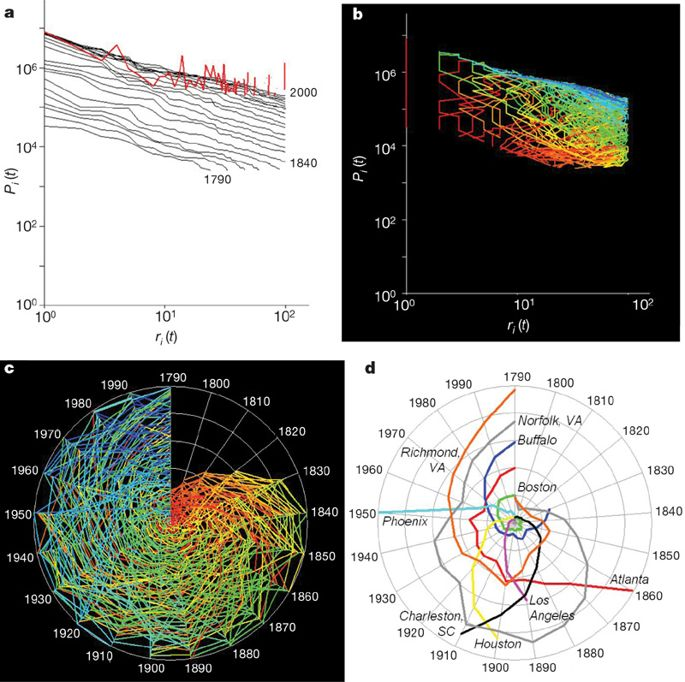
\includegraphics[width = 0.9\linewidth]{pictures/rankclocks.jpg}
    \caption{出自\cite{Batty2006}。图(a)是每个 Zipf 图。每条线代表一年的城市排名与城市规模的关系。红色线是1950年的城市排名与2000年的人口构成的点对练成的线。(b)是不同城市位序随时间的变化规律。(c)则是序时钟。每个点到圆心的距离代表它的排名。(d)图是几个城市的序时钟轨迹。}
\end{figure}

我提出了一种解释城市兴衰演变的机制。并在我之前提及的生成模型中加以使用,得到了很好的结果。该模型进而解释了城市多中心的出现以及城市收缩\cite{martinezfernandez2012shrinking}现象的出现。在已知的统计物理模型中,城市系统在空间限制和经济投入限制下的动态演化机制还是一个较少被理解的话题。本文中借鉴了空间网络中的匹配增长模型的思想方法和随机过程中的尤尔西蒙模型框架,提出了空间尤尔模型(spatial Yule model,SYM),来考虑城市的生成机制,以期达到在有足够随机性的前提下得到城市的空间分布的一般模式。

我们考虑逐渐一个逐渐出现新城市的方形空间。与此同时,人口也逐渐地加入这个城市系统中。但是只可以加入已经存在的城市中。由于城市的加速生长属性。我们认为,每个城市中的新人,都是一个已经在这个城市定居的人带来的,所以它们定居的位置会在已经定居的人的一个邻域范围内。为了建模的方便,我们认为,这个位置就是前人定居位置的一个随机方向上的一个固定步长所确定的位置。接下来我们要描述占领机制。由于有自上而下生成城市的假设存在,以及行政区划的限制,我们认为一个城市的人口在占领了一个区域之后,这个区域的归属权就不会易主了。而在模型之前的假设中,每个人又只是一个质点。我们需要给他一个可以控制的最小区划单元,来作为占有机制,排除其他城市的侵占。所以我们将空间分为$N\times N$个小方格,也即将空间打上横N纵N的线。这种操作也相当于假设每个格子的长宽都规定为1。每个格子归属于哪个城市,取决于落在其上面的第一个人口的户籍所在。在此之后,如果新的同城市结点落在这个格子上,那么它就可以生存下去;而其他城市的结点落在这个城市的区域上的时候,则会立即死亡。也就是说,我们给了这个模型的区域占领完全的先入优势。这也是经济学中常见的假设。

最后的一个假设是模型的关键。对于一个区域的建设来说,通常有一个建设的瓶颈,即来自上层的经济投入。比如说,对于中国来说,近些年来的经济增长上限一直是比较固定的。在全球经济环境的限制下,我国的GDP年增幅一直在$7\%$左右。也就是说,我们在每时每刻创造的财富的价值是有其上限的,并不能随着时间单调递增。而在本模型的考虑中,每个新的人口加入城市所需要的培养成本可以认为是相同的。于是我们增加一个“记忆核”的限制,使得只有有限个结点可以产生子结点。即每个人加入我们考虑的空间的时候,要先在这个记忆核中“登记”,再加入这个空间。而这个记忆核的大小是有限的,我们记它的大小是$N^*$,那么如果记忆核已经被填满了,新结点的加入,就会挤出一个旧结点。这样就相当于对系统的生长增加了一个经济指标的限制。从而使其更贴近现实。

该模型可以解析地导出区域内城市规模地Zipf分布;单中心城市人口密度的Clark分布;以及城市边缘的分形行为。但是我们不满足于此。记忆核机制相当于制作了$N^*$枚金币。在城市人口很少的时候,每个来城市淘金的人都能分到一枚金币。他们也可以用这枚金币在城市的某个地点买一层房子。随着时间的流逝金矿逐渐被耗尽。新加入的人就只能从已有的人的手中拿金币来在城市某处安家。我们以空间为研究对象的话,金币的空间分布可以理解为社会财富的分布。在开始阶段,大家都围绕着城市中心转。在后期资源开始不够了,边缘地区的金币由于密度低,就更容易消失殆尽。进而导致城市收缩。当然,这个过程也有着一定的随机性,导致旧中心转移到了新的中心,或者旧中心保留的同时,城市出现了新的中心。总之,在这个模型中,城市多中心现象和城市收缩现象都是由于有限的社会资源在空间上的配置问题。
\chapter{城市内部复杂现象的物理解释}

我们长久以来知道城市的优势在于规模效应。城市增长与发展规律就成为了研究城市命运的一个重要内容\cite{thisse2010toward}。Bettencourt和West在\cite{bettencourt2010unified}中讲述了城市优势的具体形式:超线性增长,即城市指标的增益随城市规模的增加呈现超线性的趋势。Barthelemy在\cite{Barthelemy2019}中讲述了城市结构的诸多方面,既有好的方面,比如城市的创造力\cite{Arbesman2009};也有坏的方面,比如城市中传染病的发病率\cite{PhysRevE.94.052316}和犯罪率\cite{banerjee2015competitive}也在城市规模增大的过程中增加了。

\begin{figure}
  \centering
  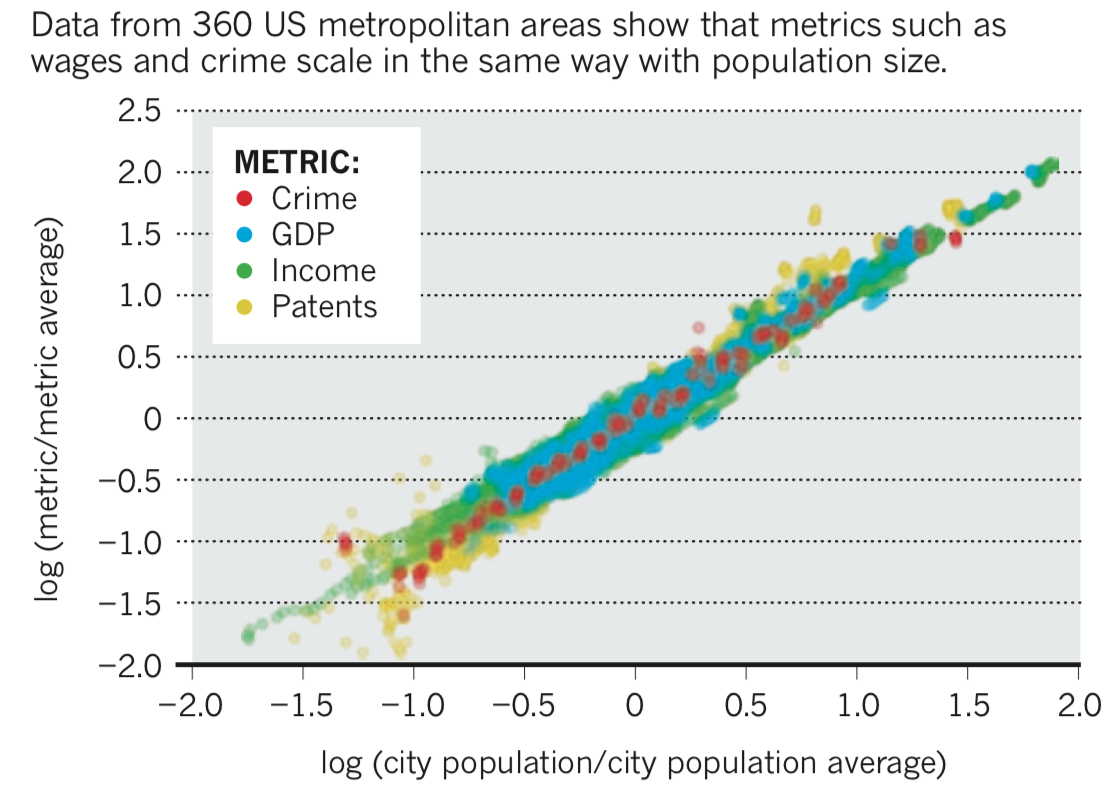
\includegraphics[width = \linewidth]{pictures/scaling.png}
  \caption{Bettencourt和West\cite{bettencourt2010unified}。360个美国城市中各项指标与城市人口之间的关系。我们可以看出,城市越大,无论是商品,资源还是观念,普通公民拥有,生产和消费的东西就越多。平均而言,随着城市规模的扩大,人均社会经济数量,例如工资,GDP,生产的专利数量和教育和研究机构的数量都在增加,而且比预期的线性增长高出约15%。}
\end{figure}

与此同时,城市基础设施建设是一个自上而下的,需要用有限资源覆盖尽量大的区域的问题\cite{PhysRevE.90.022803,PhysRevE.74.016117}。空间选址问题的解显示,最优配置的密度是亚线性的,即基础设施的数量的增加比城市规模的增加要慢。在\cite{PhysRevE.74.016117}中,作者讨论了在人口密度不均的国家/地区建造医院,机场或购物中心之类的设施,以使人的住所到最近的设施的平均距离最小。我们回顾了此问题的一些先前近似处理,这些处理表明,设施的最佳分布应具有随人口密度增加的密度,但其速度要比线性慢(三分之二)。该结论通常可以用两种方法来验证,即回归分析方法,和基于密度依赖的地图投影方法。不同的基础设施的能覆盖的空间面积也是不同的。不同基础设施和产业的相互支持关系使得城市功能形成了一个生态系统。每个城市在不同产业的不同层次承担了不同的任务\cite{camagni1993city,christopherson1986city}。在\cite{PhysRevE.74.016117}还提出了空间设施之间的交互问题。例如机场建设起来后,我们还需要研究机场之间的航班网络。其中处理的方法是建立成本度量,进而使网络维护和旅行的总成本最小化。这可以给我们一些经济方面的启示。在资源配置的时候,不只是资源支持人的生活,亦是资源支持其他产业的生产。

城市研究中,在空间和经济投入限制情况下的动态生长状况一直是难以预测的。我们将首先以交通为线索,讲述城市内部亚线性的导出模型。随后我们将对城市生态系统的性质展开讨论,并给出几个理想的进展方向。城市要素在空间上存在着交互。通过对城市内部交互进行建模可以得到城市的很多规律的物理解释。城市增长规律的超线性性和同级别城市基础设施建设的亚线性性就是典型的例子。但这种解释是否是第一性的还有待研究。本章试图整理空间交互在解释城市内部尺度的现象的工作,并给出一些已有结构的限制条件下,空间交互适应环境的一个优化模型。

\section{城市形态与随机几何模型}

与其他地理现象一致,城市的发展也会受到地形、已有人类活动分布的限制和影响。Courtat在\cite{Courtat2011}中所言,局部的地理环境可以被比作限制城市发展的壳。所以城市在形态学上形式各异,已知的任何模型都不能将城市的几何、功能、和动力学过程纳入统一的可预测框架之中。\cite{Courtat2011}中的模型利用街道和城市性质进行建模,假设城市的发展遵循空间划分或扩展的逻辑,并提出了一种动态模型,该模型可以模仿这种逻辑,并且可以通过简单的一般规则和一些参数成功地产生大量的城市多样性并重现静态分析所指出的一般特征。

这一工作将城市简化为街道段地图,并表明我们可以基于这种几何与拓扑表示推导出很多城市信息,而无需人口分布、街道宽带等的附加数据。当我们将城市当作一个图来理解时,我们可以挖掘出城市的几何特征,其拓扑特征可以作为构建城市形态的骨架。尽管城市总体形状不同(一阶拓扑各向异性),仍存在一些基本的规则可以解释城市的普遍形态。城市基础设施的分布适应于不同地区的局部地理环境,满足当地人们的居住需求并同时保持高效的城市通行。这一工作提出的基于空间划分或扩展的模型提取了超越局部因素限制与动态行为的城市结构特征。例如,生成的街道系统的对数缩放具有全局性和非平凡属性,可以验证模型并适用于观察到的较小的拓扑半径中。城市形态的生成过程实现了对空间的划分和扩展,通过模型的调整和结果比较,验证了这一过程对城市建模具有鲁棒性。

空间尤尔模型在这个问题中也有着很好的对应。如果我们将模型中的占领机制忽略掉,在时间趋于无穷的时候,二维欧氏空间上的单个社区的生长会趋向于一个圆盘的形状。但是,如果我们考虑空间占领的机制,情况就会发生改变。这使得几个区域之间的边界呈现出分型模式。这也与国与国之间形成的自然边界是类似的。所以空间尤尔模型的局部博弈机制也可以解释区域之间边界的分型特征:这些是由确定了具体归属的微观层面的竞争机制导致的。

另一方面,不只是城市景观,城市活动在空间上也存在者分异性特征。\cite{hierarchicalorganization}给出了一种结构指标。这种结构指标给出了人类移动性和城市宜居程度的关系。更强流动性的城市的市民使用公共交通的比例更高,城市功能更加分散,城市更加扁平,宜居性也越强。

\begin{figure}
  \centering
  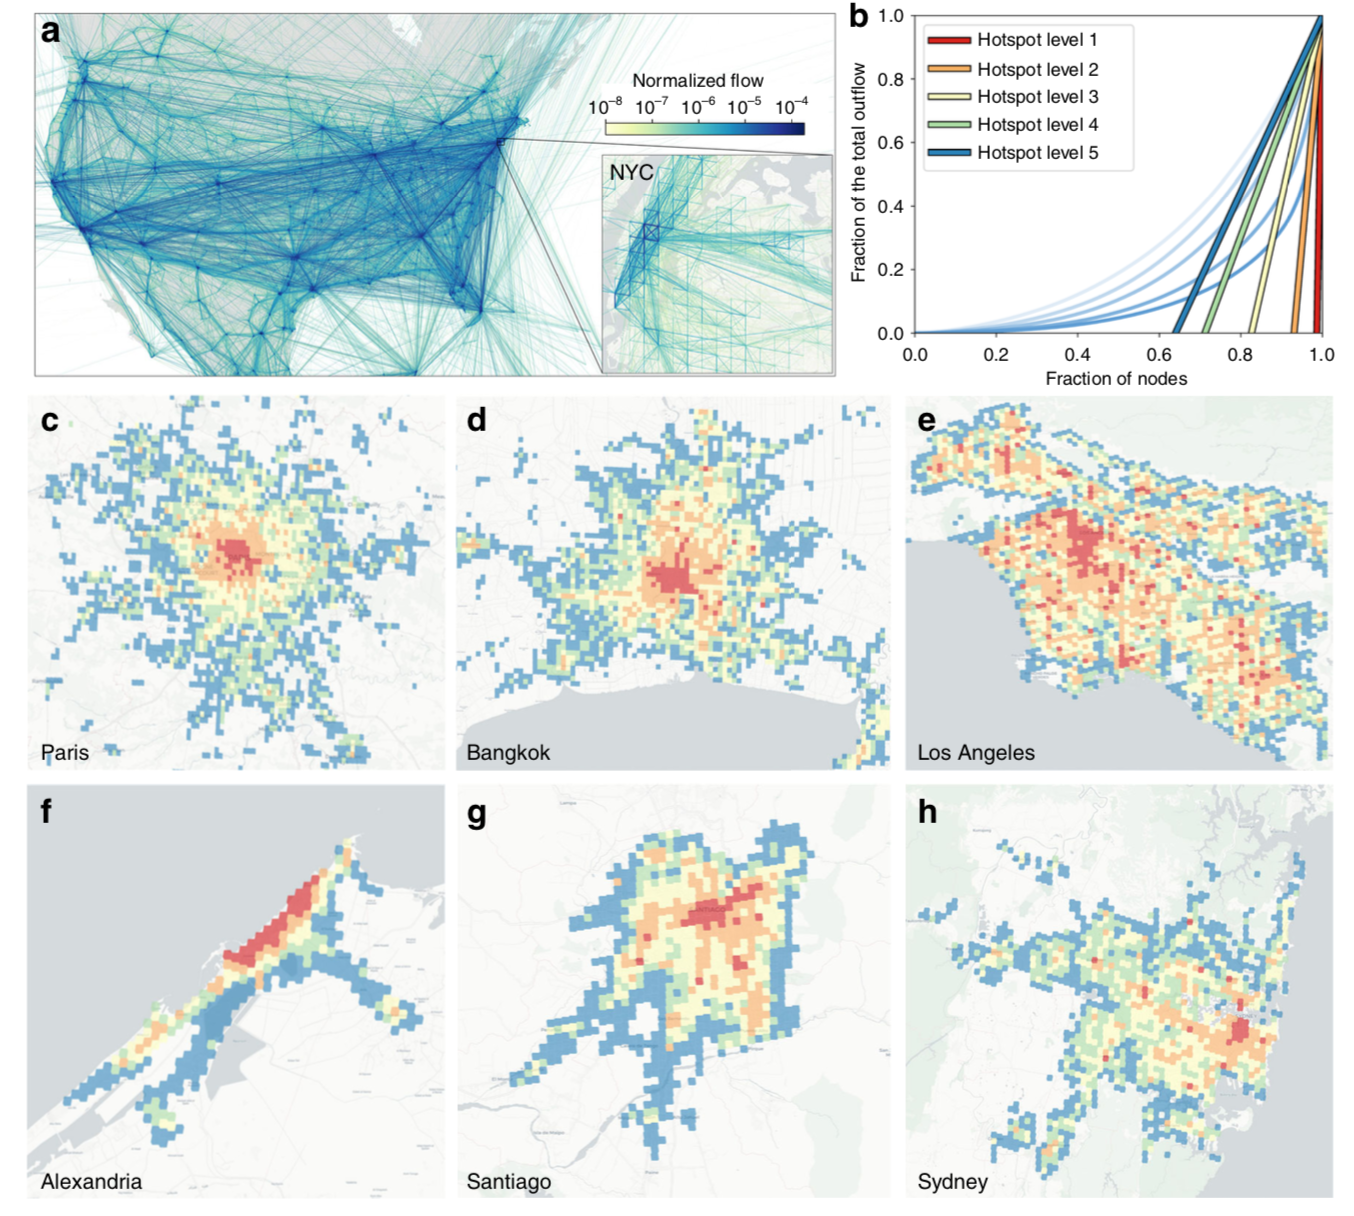
\includegraphics[width = \linewidth]{pictures/h1.png}
  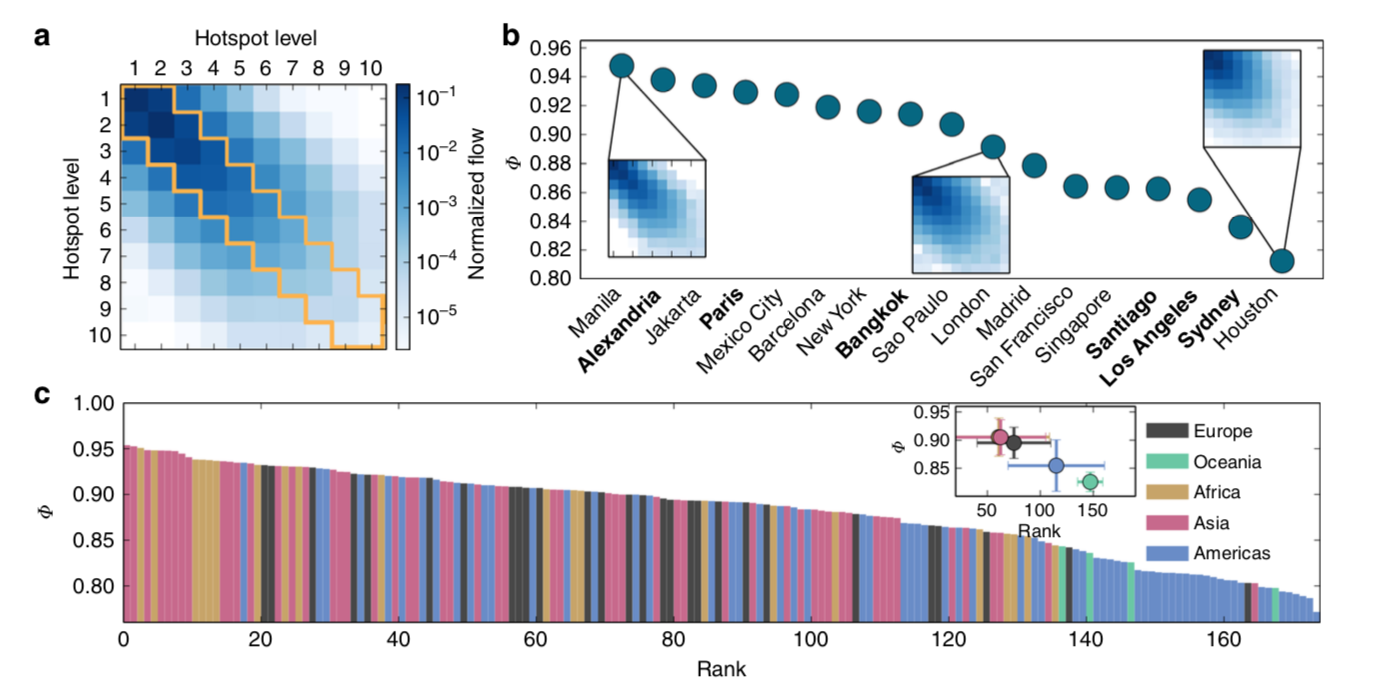
\includegraphics[width = \linewidth]{pictures/h2.png}
  \caption{上图是城市热点分析。下图是城市热点层级结构与\cite{hierarchicalorganization}中指标的相关性。文中进一步解释了集中性与城市宜居性之间的负相关关系。}
\end{figure}

\cite{Weiner17874}中的模型描述了自然竞争机制下空间分异和异质性人群演化的规律。模型中不同群体占据不相重叠的空间,而营养物质则在空间中随机扩散。结果表明:养分扩散速度是生物多样性和人口变化的时间尺度的重要参数。营养物质的快速扩散使某些物种的种群移动的收益为零,从而导致物种灭绝。此外,领土竞争会自发地产生多重稳定性,因此小规模的扰动会对生态产生重大影响。空间中对资源的竞争使得更多的种群可以共存。这个数学模型在理论上解释了城市复杂的形态和高速的流动性使得城市尺度上可以保留产业的多样性。

城市空间分隔也存在着一些物理背景。1971年,Schelling提出了一种模型,如果有太多相反类型的邻居,他们的家庭就会搬家。在\cite{Durrett14036}中,考虑了模型的一个总体种群版本,其中将一个城市划分为N个街区,每个街区都有L座房屋。对于某些$\rho <1/2$,有$\rho NL$红色种族和$\rho NL$蓝色种族。如果邻里有对等类型的$≤\rho cL$个家庭,他们会感到幸福,否则,他们会感到不高兴。每个家庭搬到每个空置房屋的速度取决于他们当前所在位置和目的地的幸福感。我们的主要结果是,如果邻域较大,则将存在临界值$\rho b<​​\rho d<\rho c$,因此对于$\rho <\rho b$,这两种类型会随机地均衡分布。当$\rho >\rho b$时,出现一个新的隔离平衡。对于$\rho b<\rho <\rho d$,存在双稳态,但是当$\rho $超过$\rho d$时,随机状态不再稳定。当$\rho c$足够小时,当$\rho $接近$1/2$时,随机状态将再次成为平稳分布。如果是这样,则在其之前是双稳态区域。该工作的结果显示,城市空间物理分隔的机理性解释不一定存在。不同的城市模式可能只是相同的初始状态被轻微扰动后得到的模式。

Makse, Havlin和Stanley在1995年引领了Diffusion-limit aggregation(DLA)模型在城市科学中的研究\cite{MakseModelling}。该模型认为城市的增长方式可能类似于二维粒子聚集体的增长,也有几篇工作\cite{doi:10.1111/j.1538-4632.1991.tb00245.x, BENGUIGUI199513}使用聚类统计物理学的思想对城市增长进行建模。DLA模型预测应该只存在一个大的分形城市,并且可以不使用传入的“发展单位”(例如,代表人员,资金或资源),因此集群的几乎所有增长都发生在城市边缘的尖端。该工作改进了DLA模型。其中与发展单位相关而不是随机添加到集群中的模型,能够更好地再现观察到的城市形态和城市中子集群(“城镇”)的区域分布系统,也可以描述城市增长动态。该模型与存在密度梯度时的相关渗滤模型相对应,其出发点是城市地区的发展吸引了进一步的发展。该模型提供了预测城市形态的全局属性(例如标度律行为)的可能性。

笔者对城市仅在边缘生长和城市自然生长进行了数值模拟,得到了相似的模式图案。
\begin{figure}
  \centering
  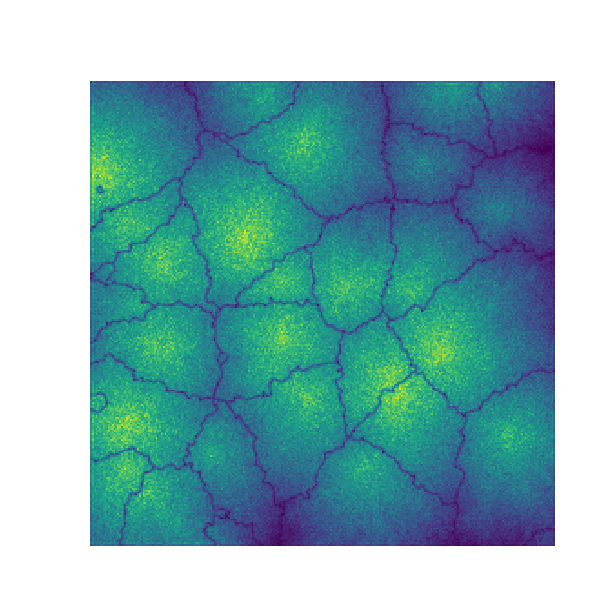
\includegraphics[width = \linewidth]{pictures/fractal_41_256.pdf}
  \caption{仅仅假设边缘增长情形下,由SYM模型生成的的城市模式。浅色代表高人口密度。}
\end{figure}

\section{城市交通系统的性质}

城市交通系统是理解城市内动态的重要切入点。从短时间尺度来看,交通可达性决定了城市建设可能的通行范围,交通拥堵的舒缓的理论解释也是所有人关注的焦点之一;长时间尺度来看,交通网络可以联系物质空间上的价值分布,所以交通网络的性质对塑造城市形态,尤其是多中心性,有着重要的指导意义。

城市交通系统是难以研究的。以路面交通的单一路段来说,路段的流量与速度之间是非线性关系。增加路网通勤效率与建设成本通常也是矛盾的\cite{GulyNavigable}。我们有必要处理细微变化对交通系统的影响,所以需要引入弹性的概念。弹性在自然和工程系统中都有很广泛的应用。它表示了系统从不同的干扰中适应和恢复的能力。尽管弹性是一个在交通系统中管理风险和理解其是如何崩溃的重要概念,但是这个概念在交通系统中的定义和它的统计性质还是缺失的。\cite{Zhang8673}基于交通堵塞的时空组团,定义了城市中交通弹性的概念。并发现,在2维城市路网和1维高速公路中,弹性的概率分布是无标度的,并且有着相同的标度指数。交通弹性也揭示了时空堵塞组团和恢复时间的关系。这种关系是与微观机制独立的。

饱和交通系统的疏解也是短时间尺度交通问题的重要关注点。\cite{PhysRevE.88.054801}基于具有随机三相交通流模型进行了数值模拟,揭示了过饱和城市交通中的移动队列(移动拥堵)在交通信号“上游”的一定距离处溶解,同时转换为同步流。这种交通拥堵的吸收作用可以通过强有力的驾驶员速度适应性来解释:车辆之间的时间间隔(空隙)在行进队列(行进拥堵)的上游增加,导致移动队列被疏解。事实证明,在给定的交通信号参数下,速度适应效果越强,信号位置与道路位置之间的平均距离越短,移动队列在该位置处完全溶解,过饱和的交通仅由同步流组成。

有研究显示,城市交通系统的异质性是由不同城市景观的异质性导致的\cite{Louf2013}。不同的城市景观有着不同的吸引力。随着人口的不断流入,人们会选择对自己最合适的位置来进行就业。开始的时候人们都会选择吸引力最强的地方工作,而随着人口的增加,这个城市景观的周围也会变得很拥挤。进而其他城市景观的相对优势开始突出,人们开始选择新的城市景观进行工作。我们可以发现,这种简单的抽象保留了城市多中心性形成的自然规律。根据Fujita和Ogawa1982年的模型\cite{fujita1982multiple,ogawa1989nonmonocentric},一个人搬到这个城市,会选择住在$i,$ 工作在$j$,使得\[Z_0 = W(j)-C_R(i)-C_T(i,j)\]达到最大。自左到右是:效用,$j$的工资,$i$的租金,$i$到$j$的通勤费用。通勤费用一般来讲正比于欧式距离:$C_T(i,j) = td_{ij}$. Louf在此基础上进行了一些修正。首先,由于换工作率高于换房率,我们认为,一个人先随机找一个住处,在此条件下,再从$N_c$个工作中随机找一个。而后可以定义活跃子中心为潜在中心的子集。在此假设之下,租金就会被预先确定下来,那么$i$处定居的人找一个$j$处的工作就会要求$Z_{ij}$达到最大,其中\[Z_{ij} = W(j)-C_T(i,j)\]所以下面就讨论一下$W(j)$和$C_{T}(i,j)$两个量。空间吸引力$W(j)$可以设为均匀分布的随机变量。则$W(j)=s\eta_j,\eta$为$[0,1]$上的均匀分布。交通成本则稍微复杂一些,\[C_T(i,j) = td_{ij}[1+\left( \frac{T_{ij}}{c}\right)^\mu ].\]其中$T_{ij}$为单位时间的路流量;$c$:为路网容量;$d_{ij}$为住处$i$到工作地点$j$的欧式距离;$\mu$为堵塞的摩擦系数。下面我们认为$T_{ij}$只与就业位置$j$附近的交通状况有关。写成$T(j)$. 每一个来到这个城市的人,会先选择一个位置$i$定居。如果对于任意的$k\in\{1,2,\cdots,N_c\}$, $Z_{ik}\le Z_{ij}$他会选择就业中心$j$工作。其中\[Z_{ij} = \eta_j-\frac{d_{ij}}{l}\left[ 1+\left( \frac{T(j)}{c} \right)^\mu \right]\notag\\
l:=\frac{s}t\]假设$l$足够大,也即最大收入相对于城市规模足够大,也即经济状况足够好,使得在人口比较少的时候,每个人都可以去唯一的市中心工作(工资比较高),也就是说,经济发展水平足够好,使得中心可以出现。

我们简单分析一下这些参数的意义。单中心结构中,$\eta_j$处于绝对统治地位。可以写成$Z_{ij}\approx \eta_j$。所以在小城市中,市民都会选择到最有吸引力的位置($\eta_t$最大处)来工作。也即单中心的情形。我们以后默认$\eta_1\ge \eta_2\geq\cdots.$ 最有吸引力的结点的吸引力是 $\eta_1$。当人口 $P$增加的时候,$\eta_1$附近的交通状况会变差。这会使得单中心 $\eta_1$的优势减小,直到某一时刻,对某个新加入的居民来说,$\eta_2$是一个更好的选择。这一时刻,一定有
\[Z_{i1}<Z_{i2}\notag\\
\eta_1-\frac{d_{i1}}{l}\left[ 1+\left( \frac{T(1)}{c} \right)^\mu \right]<\eta_2-\frac{d_{i2}}{l}\left[ 1+\left( \frac{T(2)}{c} \right)^\mu \right] \]我们分析一下上面的式子。现在所有人都在唯一的中心工作。所以$T(1) = P,T(2)= 0.$ 由于$i$是随机选取的。所以我们认为$d_{i1}\sim d_{i2}$. 为了计算的方便,直接令$d_{i2} = d_{i1}$. 另外,不妨假设各个区域的工资水平是均匀分布的,$\eta_2-\eta_1 = \eta_3-\eta_2=\ldots=1/N_c$. 于是
\[(1/N_c =)\eta_1-\eta_2<\frac{d_{ij}}{l} \left(\frac{P}{c}\right)^\mu\notag\\
P^* =c\left( \frac{l}{LN_c}    \right)^\frac{1}{\mu}\]我们就找到了一个临界人口,使得城市从单中心逐渐变成多中心(如果这个值$<1$,就不会出现单中心)。根据统计分析,$T(j)$的分布是尖峰状的(前提)。所以每个中心的通行量都差不多,$T(j)\sim P/(k-1)$. 把上面公式中的$N_c$换成$k-1$,把左面换成$\max_{j\in\{1,2,\ldots,k-1\}}(\eta_j)-\eta_k$即可得到第$k+1$个中心出现时的临界人口
\begin{align}
  \frac{L}{l}(\frac{P}{(k-1)c})^\mu>\max_{j\in\{1,2,\ldots,k-1\}}(\eta_j)-\eta_k\notag\\
(ave({\eta_1-\eta_k})=\frac{k-1}{N_c+1})\notag\\
\bar P_k = P^{*}(k-1)^{\frac{1}{\mu}+1}\notag\\
k\sim(\frac{\bar P}{P^{*}})^\frac{\mu}{\mu+1}
\end{align}
最后一个公式的意义为,人口为$\bar{P}$的城市里,出现的中心个数是人口的亚线性函数。这个结论,对于其他的城市资源也是成立的。我们可以认为城市中的亚线性现象的根源是景观优势对于可达性困难的相对强弱。

研究推进到这里,我们可以进一步讨论总通勤距离的性质。根据以前的研究成果,总通勤距离是人口的亚线性函数:$L_{tol}\sim P^\gamma,\gamma\in [0.5,1].$ 原作者解释:城市既不是有中心结构,又不是无中心结构。亦有其他说法,说从古至今,人类能容忍的总通勤时间是每天一个小时。我们将这两个结论结合起来,可以得到技术进步的速度。但这其中有多因素相互影响的问题。此处无法讨论详细。\cite{Louf2013}中得到的启示叙述如下:每个中心都可以理解为一个场的源。在位置$i$的结点会选择在此处势能最大的中心工作。同时,这个操作会对该中心代表的场起到副作用。从而存在某一时刻,存在一些位置,其他场的势能大于该场,新加入的市民连接到其他中心。这意味着如果我们假设整个城市在$k$个独立的场上。那么均衡状态就是新加入市民以等概率连接到这$k$个场源。也就是每个中心的交通在次序统计量的意义上,拥堵情况是相同的。(吸引力相同,则$Z$相同;$\eta$是同阶的,那么$T$也是同阶的。)新加入的市民会依照家地理位置和到中心的距离来选择工作地点。那么,当一个新中心刚刚建立,它的$T(j)\approx 0.$ 她就有很高的可能性选择新中心作为工作地点。这种情况会一直继续,直到最后一个中心也同样拥堵,再有结点倾向于在新的中心工作。

Louf和Barthelemy在\cite{Louf2014}中证明人口密度取决于每天行驶的总里程数,路网的总长度,总的交通延误,总的汽油消耗,二氧化碳排放量以及面积与面积之间的关系。城市人口都由一个单一参数控制,该参数表征了对拥堵的敏感性。拥挤有关的经济损耗与人口规模呈超线性关系,这意味着尽管城市中存在多中心趋势,但其交通基础设施严重依赖于交通敏感模式的城市是不可持续的。定量地来说,人口数与城市汽车的单日总里程是幂律关系。$P^*=c(\frac{l}{\sqrt{A}N_c})^{1/\mu}$。我们可以总结:真实网络中常见的现象:在小尺度上是小世界网络,在大尺度上是幂律网络。对于道路网络的对应:切换交通工具等价于切换特征尺度。

而在城市的内部,多中心现象的出现也一直是一个不易解决的问题。已有的模型中,经常通过探究经济活动以及工资、租金在空间上的不均匀分布,在某种空间优化函数下的最优分布。但是,这些方法很难给出城市演化的一般规律。首先,这些模型将空间描述成了职业地与住宅地的静态空间分布下所达到的均衡状态。而这种刻画反映过不了城市是一个非均衡的增长系统。而其增长机制本身也是一个引人入胜的研究话题。其次,这些模型中引入了过多的变量,这些变量之间所存在的多重共线性使得模型的分析变得十分困难。而对发展过程中的不同状态的理解过程也十分不易建立。但是我们可以通过一些动态生成过程来近似城市多中心问题的形成过程。面对这些问题,我们通常采用的是人口普查的办法,对城市的大小和人口分布进行精准描述。并利用不同年份的普查数据构成的时序数据集,进行区域中人口空间分布的回归分析。这些数据集的优点是,它们以时间序列的形式囊括了人口分布的准确信息。


\section{关于路网演化的新问题}

生成模型的一个难以克服的缺点,是无法解决已经形成的结构(比如路网、建筑)在长时间尺度的变迁问题。这一段中,我将以城市内部交通路网的优化为例,叙述一个可以有效解决已经存在的路网模式的优化的问题。

汽车产生之前的城市,是步行者的尺度;汽车产生之后的城市,是汽车的尺度。这之前与这之后,东西方的城市在尺度上没有太大的差别,而尺度是城市最重要的东西。”1913年,福特公司以流水线装配T型汽车,小汽车开始进入家庭。这之后,扩大街坊、减少十字路口、建设快速路,成为欧美城市规划的新潮。这股力量险些毁掉了曼哈顿的街道——上世纪五六十年代,经市民抗争,高速路才没有被插入市中心。取而代之的是发展地铁等公共交通的计划,这使曼哈顿的传奇得以延续。在这里,城市的立面(建筑高度)不断攀升,城市的平面(街道肌理)却依然如故,城市的品质(充足的就业机会、街道上的乐趣等)一如既往;攀天大楼还与地铁保持着良性关系,前者为后者提供了客流,后者支撑了前者的生长。

北京则步入“汽车城市”的后尘。1950年代以来,它在兴建高层建筑之时,以宽大的路网,对城市的平面进行了改造:街道两侧的围墙又被修了起来,如同北宋之前的坊墙;沿街商业不再被鼓励,它们被点状分布的大型购物中心“收编”,后者如同唐代长安城的东市与西市——城市形态似乎回到了一千年前的里坊制。如此大拆大建旨在方便交通,却使北京沦为世界上最拥堵的城市之一。在这颗星球上,还没有哪个城市能以小汽车交通为主宰而获得成功。“北京与曼哈顿的故事告诉我们一个道理,”在美国国家建筑博物馆,我得出这样的结论,“城市的平面比立面重要,街道比建筑重要,交通政策比交通工程重要;人性化的尺度是一种重要的城市遗产形式。” 

我们回想一下交通系统设计的初衷:使不同位置的人可以在尽量短的时间内到达想去的位置。但是如今的交通系统里,可达性问题基本已经得到解决。而拥堵已经是最大的问题。这具体表现在:道路拥堵导致出行时间过长;群体出行时间优化与个体出行优化目标不一致;目标改变:节能减排,即优化总出行距离等等方面。我们度量交通系统的过程中,欧式距离或者曼哈顿距离已经不再是唯一的指标。更重要的方面是通勤时间的问题。对于现在城市的问题:建筑和街道建设趋于完善,重新建设难度巨大。很难根据现有的城市,通过小规模的改进如何大幅度提升路网性能。我想到的一个方案是基于这样的思路的:应该让个人出行行为向群体规划的方向进行,并建立不均衡的道路规划方案。这样做可以引出的结果就是局部形成环路,进而得到跨尺度的临界点对应网络的相变点。也就是小世界转化成无标度网络/短距离与长距离交通行为的转化点。

进一步分析这个思路。我们意识到大部分城市之中,城市的路网结构可以抽象为星形或者格网型。前者对应着明显的层级结构,后者是网络重整化常用的基础模型。路网可以进行跨尺度分析。我们对路网建模如下:有空间坐标的三元组:$\{N,E,\Lambda\}$,其中$N$代表路口集合,$E$代表路段集合,$\Lambda$代表某个单向的车道数所占比例的集合。比如双向四车道通常是左右各两车道,对应的$\lambda$就是$0.5$. 容易得到路段的流通量是车道数$k$的函数:$V_i = V_i(k)$。下一步我们要对出行线路建模为$(a_0,a_1,a_2,\dots,a_m)$,其中$a_1,a_2,\dots,a_{m-1}\in N$,即车辆从$a_0$出发,从$a_1$进入路网,从$a_{m-1}$驶出路网,最后到达终点$a_m$。随后我们就可以建立对道路双向通行的比例$\lambda$进行优化的算法:\begin{enumerate}
  \item 初始化城市路网,包括每个路段的路网宽度和$\Lambda$
  \item 通过二维正态分布(可替换)生成OD数据集,以泊松分布注入路网中。
  \item 每$\Delta t$,遍历所有车辆的位置,所有路段的速度。
  \begin{itemize}
      \item 如果路段$n(e_i)>threshold: $  更新$\lambda_i = \frac{1}{1+\frac{\lambda_i}{1+\lambda_i}}$
      \item 对称地,找到$e_i',$使得$V(e_i')/n(e_i')^\alpha$,松弛反向路网。
      \item 重新对每辆车的出行进行规划。
  \end{itemize}
  \item 如果一辆车到达了目的地,则从路网中删去。
  \item 如果$\Vert \Delta\Lambda\Vert_2<\epsilon,$ 结束循环。
\end{enumerate}
这样我们就得到了一个保持原有路网形态特征,但能在一定程度上改善路网状态,形成中尺度空间的优化模型。


\section{跨尺度模型、生长模型的记忆效应}

这个部分里,我们主要叙述与尤尔西蒙模型相关的生长机制。尤尔模型最早见于对种群数量分布的解释\cite{yule1925ii}。空间依附效应是尤尔模型可以解决人口分布问题的一个出路\cite{Willis}。城市规模研究发现\cite{Keuschnigg13759},集聚效应(大城市的产出高于预期)遵循跨行业数据中鲁棒的“超线性”关系。但是我们还希望这种模式可以预测的更多的领域,涉及各个城市在许多时间点的动态标度律,我们还期望随着城市人口的增长,各个城市之间出现平行的超线性增长。

根据第二章最后提出的理论,城市收缩是因为到达了环境上限。这个模型还可以反映出城市的加速增长机制,以及在空间和经济资源的限制下,城市发展的上限问题和极限情况。我们可以得到一些合理的推论。比如现在的城市发展过程大概处于本文所提出模型的初步阶段,绝大多数的区域并没有呈现出明显的空间挤压效应。然而,在全球的几个著名大都市区中,我们利用夜光数据集给出的验证结果显示,近几十年的快速城市化和人口激增使得很多城市面临了很大的空间限制。经济资源的限制只在很少的地区得到了证实。

城市的发展是历史累积的,是在高度异质性和差异性的环境中不断演化的。而生长模型中,如果将大多数机制建立在无记忆性的指数增长过程中,模型对于复杂历史状况的城市演化规律的解释能力就会有所下降。生长模型本身的研究过程也在不断引入新的改进机制,从而使得模型仍能预测出较为确定的指标(可解析性,以及更多的考察要素,如Taylor定律\cite{Giometto7755}。),也能得到更符合实际状况的预测效果。不过这些结果无法超过环境容纳量的上限。如何解决这个抽象的上限的问题则是我们下一章要讨论的内容。即城市生态系统是如何运作的。
\chapter{开放城市系统}

城市的组织是复杂的。我们经常用模糊场所来描述不同空间区域在城市中所承担的分工。而一个空间位置也可能同时从属于不同的场所。城市科学的研究对象与生态系统有着类似的性质。在生态系统中,多个组分相互作用导致各自在系统中的种群密度发生变化变化。在城市中,市民对居住条件、工作条件的要求,企业对物流链、地租、工作环境的要求,也使得城市区域分化成了有一定特征的模式。在\cite{christopherson1986city}中提到了一种观点,称城市为一个工作站。这是因为城市是一个集合了各种工具,并由于其中复杂的相互依存、相互促进的关系而演化形成的生产单元。

这些复杂的城市元素在空间上的交互关系经过一定程度上的抽象,可以理解为城市功能在空间上涌现、迁移、或消失而组成的过程。这个过程与人类移动性\cite{molas2017field,gonzalez2008understanding,song2010limits,song2010modelling}的研究有一定的不同。城市功能的功能更具有确定性,空间特征更加明显。同时也更不可逆,是不同于基本的元人口生成模型的,也有必要单独进行建模研究。举例来说,根据\cite{banerjee2015competitive},城市标度律的形成并不一定是简单的规模效应的产物,也有可能是多方博弈的结果。以犯罪的超线性为例:默认的假设是,犯罪的超线性扩展与其他城市属性一样,是由于规模效应而产生的(也就是说,犯罪分子之间更多的联系会增加犯罪的收益)。但是,我们通常忽略的一个事实是,犯罪的发起与城市人口呈线性关系,执法人员的数量与城市人口亦呈线性关系。在\cite{banerjee2015competitive}的模型中,犯罪与执法的博弈机制成功复现了上面的标度律机制。并且该模型亦能解决某些特定类型犯罪的线性标度行为。可见,基于微观元素交互的空间模型有着比依附型生成模型更加丰富的内涵。

我们将城市考虑为生态系统的时候,城市间的流就是绕不开的问题。不同城市之间有着不同的产业分工,它们形成的生态系统使得它们可以通过物质联系来得到支持每个城市生存的生产资料。这样每个城市就可以拥有自己的特长和分工,进而在满足自身生存需求的同时不必样样精通来浪费不必要的精力。研究城市之间物质流动就成为了城市科学在城市间尺度的一个有趣命题。同时,城市之间的良性和恶性竞争也会导致政府制定的发展策略的不同,进而产生博弈行为。城市要为最多的人提供长期有效的生存条件,所以城市经济体的复杂过程要兼顾多样性与稳定性。进而城市系统的博弈与演化规律也是我们需要研究的重要一环。

现代城市空间通常不是自然涌现的,而是经过谨慎规划的、较为规整的图案。传统经济地理研究中,对城市规整性研究主要在于定性分析\cite{colonna2002proposal}和街道生成模式\cite{barthelemy2008modeling}。路网的建模主要基于结点连接的复杂网络。而实际上,这些研究的地理基础依然有待确认。空间网络的建立隐含了路网空间和二维平面等价的假设。而在一些研究中\cite{DURRETT1994363}已经证明,并非所有的空间关系中,建立空间网络与在连续时空建模都是都是等价的。只有在确认交互性质的空间网络中,离散网络的连续化才是有意义的。

而在更大的尺度上,每个城市的形成是空间资源向中心集聚的过程\cite{keuschnigg2019urban}。所以,城市之间的距离经常不是空间优化的结果。这带来的后果就是城市群自然而然的有着拓扑网络的特征。这个过程中的一些特定规模是很重要的。城市的整体意义是,大部分的沟通需求可以在一天之内完成。这给了城市功能区的组织一些客观限制\cite{schwanen2002travel,gordon1989influence}。另一方面,随着交通工具的进步,通勤速度的增加使得城市可以容纳的空间更大。更多的居住区带来的基本需求的拓展(如餐馆、公园)在空间上体现出了复杂的形态。这也可以看作是新城市聚落的形成。事实上,在生态学上有对聚落形成的理论,关注了局部生态的稳定性和可持续发展性\cite{nowak1992evolutionary}。近年来的一些新理论\cite{PhysRevLett.122.148102}表明,不同个体之间的竞争必然会导致所谓“公地悲剧”\cite{hardin1968tragedy},但合理的调控和空间纵深可以给这种现象一些缓冲。我对此的理解是,虽然复杂产业结构下的城市衰退是一定会出现的,但是这只是自组织城市体系经济周期的一个部分。这种有周期的变化比竞争性环境的确定性损失要优异的多。这也是城市设计者应该注意控制的城市结构状态。

本章将讨论空间演化博弈模型建立的理论基础、社会网络的结构与广义的共存与嵌套问题、以及大型系统的稳定性准则。在本章的最后,我们介绍了永续公地悲剧模型的工作。我们期望本章的工具与结论可以揭示:空间作为一个独立的维度,比网络性质有着更丰富的内涵,不能完全用点线模型进行抽象;我们也希望本章的内容可以给时间地理学一些新启示。

\section{空间多主体行为的分异性与共现性}

我们首先来考察如何将空间对象抽象成网络。网络可以看作是空间对象的同质个体之间的关联模式。进而一个定义良好的网络抽象应该自然而然是无标度的,因为抽象尺度应该与问题本身是无关的。这个理念的正确性保证了“采样”在复杂网络研究中的有效性。与此相关的是\cite{PhysRevLett.107.158702}中的一个重要观念:将复杂系统简化为最简单的形式,同时保留其重要属性,有助于独立于其性质对行为进行建模。我们认为,抽象出来的网络可以构建对不同是一个普适类。偏好依附(preferential attachment)就是一个重要的普适类。这个机制可以解释各个领域中富者愈富的情形。

城市生成模型通常建立在均值空间的假设之上。但是一些基于格点空间的模型(如Ising模型、Schelling模型\cite{stauffer2007ising})表明,只要个体轻微偏爱和同色的邻居一起生活,社会也会发生完全隔离。真实情况下,居住区尺度的种族聚集现象也是真实存在的。所以在研究区位分异问题时,均值空间的生成模型并不能取代固定位置的交互模型。具体的,\cite{DURRETT1994363}一文建立了离散的空间模型在人口动力学中成立的理论基础。四种对空间分布系统动力学进行建模的方法:平均场方法(用常微分方程描述),其中每个人都被认为具有与其他每个人互动的可能性相同;小团体模型,将离散的个人分为小团体,而无需其他空间结构;反应扩散方程,其中最小个体分布在空间中;以及交互作用的粒子系统,其中个体是离散的,并且空间被明确地表示出来。文章将这四种方法应用于空间分布种群中物种相互作用的三个示例,并比较它们的预测。每个代表关于生物学的不同假设,因此,它们之间的比较具有生物学以及建模上的含义。在第一种情况下,所有四种方法都一致,在第二种情况下,空间模型与非空间模型不同,而在第三种情况下,具有离散个体的随机模型与基于微分方程的随机模型不同。这说明了离散建模对于与粒子系统相关的极限反应扩散方程可以具有与简单地将扩散项添加到平均场方程而获得的不同的定性行为。

一套严格的数学理论来解释弱自然选择机制之下的空间博弈理论。所谓弱自然选择,指的是各种策略的收益差别不大。分析的关键在于,如果合理地重标度时间和空间,那么空间模型就会收敛于某个偏微分方程(PDE)的解\cite{nanda2017spatial}。这种方法可以用来分析 $2 \times 2$ 的博弈,但还有一些 $3 \times 3$ 的博弈的偏微分方程极限是未知的。本文中,我们给出了一大类 $3 \times 3$ 的博弈的确定行为,并通过模拟验证了规律。总之,空间的效应等价于改变收益矩阵,并且只要这个过程确定,空间博弈的行为可以由复制方程来预测。具体来讲,优势策略的演化规律为\[\frac{du_i}{dt} = u_i (F_i-\bar{F}),\notag\\
F_i = \sum_j G_{ij}u_{j}\notag\\
\bar{F} = \sum_i u_i F_i\]其中\(p(x)\)为$x$与邻居的交互概率。策略是时间和位置的函数:\(\xi_t(x)\)。而策略的选择则是依据某个位置的健康程度\[\psi_t(x) = \sum_y G(\xi_t(x),\xi_t(y))p(y-x)\]来确定的。此类模型新颖的点在于:进化的角度是个体策略。即一个企业在一段时期内的动态选址的问题,在Schelling模型的背景下,就是一类弱选择演化博弈方程的解。


人类局部交互模型的通常假设是短程交互和长期迁移的组合\cite{rybski2009scaling}。短程交互的例子在植物界有很多很好的对应。草原与树林的演化规律就是自然界常见的例子\cite{durrett2018heterogeneous,durrett2009coexistence}。作者利用非同质空间上的Lotka-Volterra模型导出了二者可以在指数级别时间共存的事实。并且在初始转换之后,二者分异会十分明显。每个个体(agent)有一定强度的个人属性,这个属性可能会被其他人影响,进而发生改变。这个例子与工农业城市的演替有着很多相似之处。短程-长程结合的一个例子是人类方言的变迁过程\cite{PhysRevX.7.031008,seoane2018coexistence,PhysRevE.99.032305}。某种方言的掌握者在搬迁之后会保留一部分原来方言的特征,同时学会新的方言。

局部交互的方法通常由简单交互过程(基于Ising模型)或者博弈分析(基于纳什均衡)\cite{grimalda2016social,Mussa2019Urbanity} 来得到。Schelling引入了社会科学中最早的基于主体模拟的模型之一。 这个模型已经被社会科学家广泛讨论,并被物理学家使用与双相Ising模型和其他系统的类比进行了分析。\cite{Durrett14036}研究了元人口版本,该模型模拟了将城市划分为邻域的过程,并且进行了初步的分析,从而给出了有关均衡结构的详细信息以及密度的明确公式。空间演化博弈\cite{nowak1992evolutionary}是一种基于元胞自动机的生物数学博弈模型。这一模型通过利用按照博弈规则进行演化的细胞自动机,来获知个体的背叛怎样在未来影响群体的合作-背叛状况。该模型可用于研究细菌、社会等系统模型。对于城市模型中,我们已经确立了一些条件\cite{DURRETT1994363},使其等价于连续场模型。进而使得这种方式建模在解析上和直观模拟上都很有说服力。

% 近十年来,学界对生成模型的研究不仅仅限于联系的建立,更在于社会网络功能的形成。由于社群结构可以被看作城市生活的基本单元,进而划分空间集聚和空间异化效应的特征尺度,社群结构的定义与性质成为了一个很重要的研究对象。我们重点考察的有两个方面,首先是社会网络的层级结构(Hierarchy),其次是社会网络的社群形成规律。



\section{城市要素交互的复杂性}

城市要素交互是城市生态系统的重要问题\cite{duneier1999talking}。工业生产的协同、购物区与餐饮区的耦合、矿业区与住宅区的相互排斥等关系使得城市要素的分布需要依照一定的目标进行优化。但是现有工作对该问题的理解层次主要停留在单一属性场所的网络层次。这种方式的固有问题在于,它的表达力是基于两两交互关系的。而社群结构(群体关系)代表的不只是两两关系的叠加,而是社群固有的其他性质\cite{durrett2019probability}。空间网络的优势在于将这种群体关系固有地刻画在空间结构中。\cite{PhysRevX.4.011008}中建立的模型同时生成了一个国家内人们的地理分布及其复杂的人脉关系,将局部的人的联系建立起来,并给出一定的长程联系。\cite{PhysRevLett.123.208002}质疑了随机游动假设下的城市物质分布模式。在固定空间设施的条件下,人类的行为更类似于列维飞行。这些研究体现的都是固定空间要素的情况下,交互并不能由单一机制的方式构建起来。城市要素的交互实际上是依赖空间的。

由于网络建模的特殊性,传统的空间网络模型只能刻画空间对象之间两两的关系。近几年的一些研究\cite{newman2016estimating}开始注意复杂网络社群结构的提取和实际意义。这些研究表明,由于复杂网络的离散性,不太可能存在很完美的全局跨尺度性质\cite{PhysRevE.83.066116}。层次结构往往对应着特征尺度\cite{verma2016emergence},所以寻找城市空间里的层次结构也是使得网络抽象的思路更加合理的方案之一。对于网络来说,社区识别问题就是将大网络分割成小而稠密的子网络,使得社区之间只有稀疏的连接。社区分割是无监督问题,我们需要在开始给定待划分的社区的数量。\cite{newman2016estimating}采取的原则是最大化合适的生成模型下的观测社区结构的似然函数的方式,以得到最优的社群结构。事实上,这种方式给出了网络建模的一个特征尺度:在这个尺度上,用于网络中结点的实体的能最好地反映整个网络的介观性质。假设一个网络是有社区结构的,那么它将是这样生成的:存在$k$个潜在的社区,每个结点以一定的概率分布依次加入某一个社区。社区结构内部的结点,建立连边的概率较高;社区结构之间的结点对建立连边的概率比较低。文中模型假设结点加入社区$r$的概率:$\gamma_r\ \ (\sum \gamma_r = 1)$。如果两个结点分属于社区$r$和$s$,那么他们之间连边的概率为$\omega_{rs}=\omega_{sr}$。连边概率可以构成矩阵$\{\omega\}_{k\times k}$。如果该矩阵对角线上的元素比较大,我们就可以构造出一个通常意义上有社区结构的网络。\cite{hebert2011structural}提出了结构偏好依附的机制,这带来了一个观测复杂网络的新视角,即直接引入社区(在结点和边之外的视角)。这个模型可以通过预测其社群结构来复现社会和信息网络。更重要的是,结点和社群是如何连通的。而这通常是一个自相似的结构。

但是这些方法的表达力仍然是有限的。城市要素本身存在空间特征。如何将网络性质与城市中的距离衰减原理和城市含义中的一些基本要素(单日可返回范围)结合起来是一个值得思考的问题。


\section{城市生态系统的稳定性条件:层级结构与共存关系}

由于城市的形成是空间资源向中心集聚的过程,城市之间的距离经常不是空间优化的结果。这带来的后果就是城市群自然而然的有着拓扑网络的特征。社会网络的层次结构有着本质的空间特征。生态学中最初的层级结构就是用空间实例来描述的:岛屿上物种的类型是随着岛屿与陆地的距离而递减,因此岛屿上物种的组成是层层镶嵌的。在生物自养网络\cite{Bascompte9383}中,我们可以广泛观测到层次结构的出现。后面有一系列工作对这个现象进行了解释。比如\cite{bastolla2009architecture}说嵌套性可以减少物种之间的竞争,并且这种结构对某物种突然消亡情况下的生态系统有着鲁棒性;\cite{thebault2010stability}讲模块度(一个衡量复杂网络的module的量)和嵌套性分别产生于跨营养级和同一营养级;\cite{Allesina2012}是May于1972年工作的拓展,里面讨论了嵌套性对网络的局部稳定性是不利的;\cite{james2012disentangling}说的是nestedness就是一个伪概念,对社群结构完全没有好处;\cite{suweis2013emergence}是说用最优化的思路来看嵌套性是如何出现的;\cite{rohr2014structural}说的是嵌套性可以提高系统的结构稳定性。我们关心这个问题的原因则是为什么生态系统会出现层级结构。在地学中,层级结构可以理解为地理要素的相互依存关系\cite{PhysRevE.83.036117}。大场所圈定小场所,小场所圈定同质人口,具有哪些特征异质人口可以共同出现在同一片区域。我们知道,生态学的理论导向在于解释为什么多物种可以共存。不可共存的物种在稀释和调和能力差的区位共现时,系统就会变得不稳定。我们从两个角度讨论共存问题。分别是局部稳定性和结构稳定性。局部稳定性指的是在系统稳定的状态下给系统一个小的扰动,系统恢复原状的能力。而结构稳定性则是系统的故有状态。与物种的选取有关。

局部稳定性的讨论始于Robert May\cite{may1972will}。该文章基于Gardner和Ashby实现的计算机模拟动力系统的结论:大型复杂系统只能在一定临界程度的连通性上面是稳定的。他们的结论是基于大小为4,7,10的系统的计算机模拟研究。May在自己的工作中通过更多的变量来完善这个研究。找到稳定与不稳定的界限仍然是研究问题的关键。本实验中,作者采用的记号有:连通率\(C\),物种数\(n\)。物种之间的关系通常是非线性的。但是这样的系统都可以在均衡点附近做泰勒展开式。系统的均衡就可以由这个方程刻画:\[\frac{dx}{dt} = Ax\]矩阵\(A\)的对角线元素设置为\(-1\),这是为了考虑进时间因素。每个元素都等概率的是正数或者是负数。然后取各种值的概率都是相等的。我们将他们的均值设置为\(0\),方差的均值设置为\(\alpha\)。方差可以作为平均交互强度的代表。随机性只在选择物种的时候出现。之后的演化过程中,系统就是完全确定的了。我们有一下结论:系统是稳定的,当且仅当\(A\)的所有特征值都有负的实部。如果\(\alpha\sqrt{n}<1\),系统几乎一定是稳定的;如果\(\alpha\sqrt{n}>1\),系统几乎一定是不稳定的。相变区域的宽度正比于\(n^{-2/3}\)。我们将系统的连通度\(C\)定义为非零元素的比例。有了这个量之后,\(\alpha^2C\)就取代了\(\alpha^2\)的角色。系统稳定的临界概率\(\alpha\sqrt{nC}\)。举例来说,12物种的群落,连通度是15\%,稳定概率为0;但是3个4物种的群落,连通概率是45\%,这样的群落有35\%的概率是稳定的。这个模型的重要意义是说明了:如果将物种分组,则这种组织将会使系统更稳定。一个对应到城市的例子是:划定产业园区会使得城市经济体更加稳定。

\cite{Allesina2012}扩展了之前的结论。上面的情况是针对均衡点附近的情况的。但是自然系统中有很多不在均衡附近。但是对于大型系统来说,这种方法总是适用的。矩阵有着随机的结构(从同一个分布中得到)。这给了模型鲁棒性,但是不能刻画模型精确的混合结构。比如说,在May的矩阵中,捕食关系比共生关系要频繁一倍。注意到在大型系统中,特征值包含于复平面的一个椭圆里。圆心在$(-d,0).$ 半径为$\sigma\sqrt{SC}.$ 在稳定系统中,圆圈在左半平面。所以如果半径小于$d$, 系统就稳定:\[\sqrt{SC}<\theta =\frac{d}{\sigma}.\]比如捕食矩阵中,对称的位置符号就是相反的。在这个矩阵中,稳定条件是可以解析求得的:$\sqrt{SC}>\theta(1-E^2(|X|)/\sigma^2)$。而在竞争与共生矩阵中,又有着这样的性质:$signal\ of\ M_{ij}=signal\ of\ M_{ji}$。它导出的稳定条件:$\sqrt{SC}<\theta(1+E^2(|X|)/\sigma^2)$。对应回到城市中,一个体系稳定容纳的局部产业丰富度是很有限的。

结构稳定性的概念最早由Thom\cite{thom2018structural}提出。它的一个困难是估计取值过为艰难。很多时候只能靠模拟来估计。但由于生态系统的高端复杂性,这种估计方式有时会导致估计的结果的置信度过低。对于城市问题来说,一个有力、务实的政府是十分重要的。政策比自然恢复是更有效的解决策略。


\section{一个例子:空间公地悲剧}

虽然基于交互矩阵的生态系统结构分析已经有了比较悠久的研究历史,空间因素在生态中的真正意义还少有人解释。\cite{PhysRevLett.122.148102}给了一个空间版本的社会困境的解答。其中隐含了两层深刻的意义:生态的时间性:系统在演化的过程中存在着周期性。这意味着区域发展过程存在着势能积累。另一方面,空间性给系统提供了缓冲空间,使得势能可以积累。这与系统的弹性\cite{gao2016universal}概念是不谋而合的。这个文章的结论可以解读为:自然系统的弹性来源于系统的空间性。

城市间交互的建立是由流达成的。城市间动态平衡是我们理想的状态。但是城市发展过程中出现的很多问题也是我们不能忽视的。经济周期的出现、城市收缩、城市发展不均衡等现象的出现使我们反思,城市发展中是否有着天然的陷阱,或者是难以避免的问题。我们在追求城市发展的时候,究竟在追求什么。公共地悲剧(tragedy of the commons,TOC)是Hardin\cite{hardin1968tragedy}探索并定义的一种社会困境,它发生在两个人或群体选择不同的策略来利用有限公共资源的时候。个人出于自身利益耗尽公共资源,综合收益将劣于个体间合作、有节制地利用资源得到的利益。这种问题的根源在于人类价值观的贪念使得增加公共资源的时候,增加的生产意愿不一定会提高。所谓“三个和尚没水喝”。城市发展也有着一些对应的场景。比如说城中村、贫民窟等现象,就是城市无法使得所有人都努力工作,却提供了过得下去的生活条件,使得贫民仍愿意居住在城市之中而导致的。有一些新的研究确定了一些条件。在这些条件下,城市虽然仍不会百分百随着自身的发展而长治久安,但却能走出困境。

在宏观尺度上,TOC呈现于群体决策与环境层面,而在个体水平上,则与个体奖励机制的差异相关。由TOC困境引发的进化动力学问题可以模拟为来自两个群体(合作者和利己者)的个体频率的变化。个体间产生互动并取得收益,收益大小取决于自身及其他个体的策略,可以通过收益矩阵进行建模:
\[A = \begin{Bmatrix}
R &S \notag\\T &P
\end{Bmatrix}\]
其中,$R$表示合作的奖励,$T$表示利己的收益,$S$表示他人放弃合作而自身选择合作后的收益,$P$表示互相背叛的惩罚。TOC困境发生的条件为$T>R>P>S$。收益表示系统的适宜度,它决定了合作者(频率为$x$)和利己者(频率为$1-x$)的数量变化,可由下式表示:
\begin{equation}
\dot{x} = x(1-x)[r_c(x,A)-r_D(x,A)]
\end{equation}
其中,$r_c$,$r_D$分别为合作者与利己者的适宜度收益,可表示为$r_c=Rx+S(1-x)$,$r_D=Tx+P(1-x)$。

与标准的博弈论假设不同,TOC困境中的收益会随着反复决策过程中对公共资源的消耗而产生变化,考虑到这一动态变化,Weitz提出依赖于资源状态的回报矩阵:
\[A(n)=A_0(1-n)+A_1(n), n\in [0,1]\]
即在资源状态为耗尽($A_0$)和充足($A_1$)的回报矩阵之间进行插值,环境状态的反馈将通过$n$来实现。当$n=1$时,个体更倾向于做利己的选择,当$n=0$时,个体更倾向于合作。由于考虑了资源状态,这一系统将呈现出新的非爆炸现象——永续公共地悲剧(oscillatory tragedy of the commons, o-TOC)。

协同博弈模型可以帮助我们从个体层面理解人口噪声和空间交互对社会环境和资源动态变化产生的影响。这一模型用平均场方法导出了合作者的极限分布,同时验证了局部交互会导致空间分异的形成。由图\ref{conevol}可以看到,o-TOC呈现出持久的收敛于边界的振荡。

\begin{figure}
	\label{conevol}
	\centering
	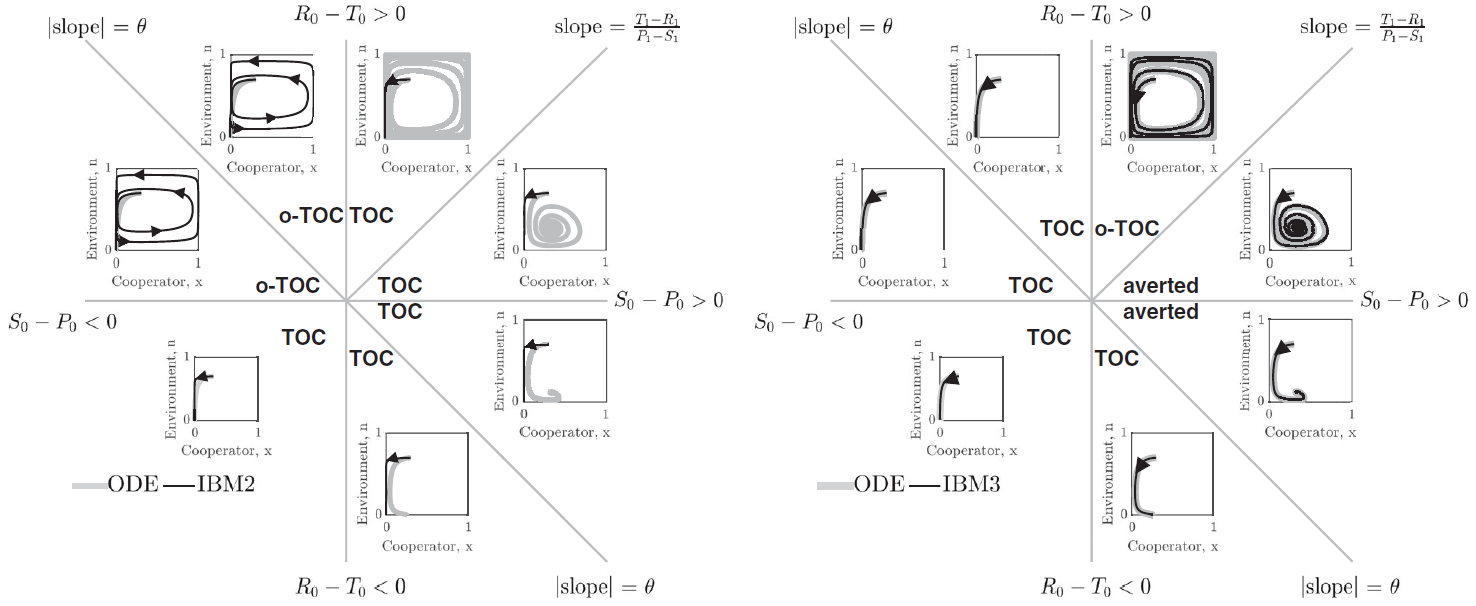
\includegraphics[width=0.9\textwidth]{pictures/Coevolutionary}
	\caption{基于IBM动态与复制器模拟的策略与资源协同进化动态。}
\end{figure}

定义扩散系数$D_n$控制相对于人口动态的资源再分配。所有情况都表现出了合作者之间的空间聚集,而在异质环境动态下($D_n=0, D_n=1$),合作者与环境资源状态间也呈现了空间聚集效应。
\begin{figure}
	\label{conevol}
	\centering
	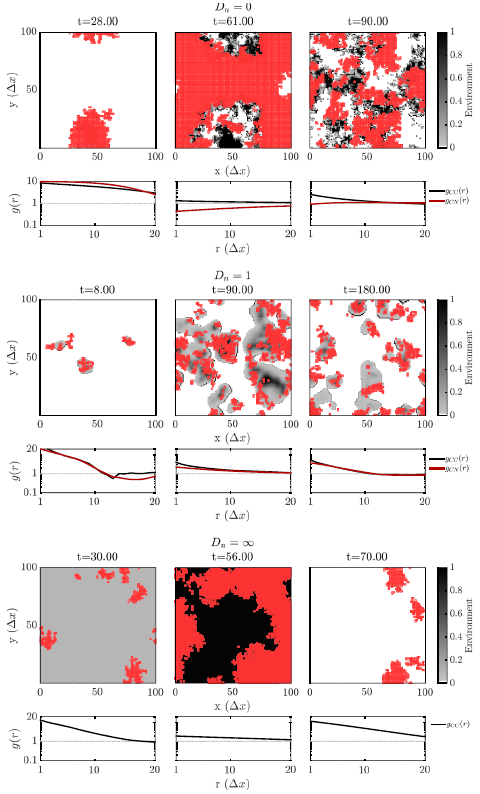
\includegraphics[width=0.7\textwidth]{pictures/D_N}
	\caption{资源与合作者的时空动态变化。背景色表示环境,红色正方形表示合作者占据的格子位置,空位被利己者占据。(顶行)$D_n=0$,合作种群的圆波向外扩散;(中排)$D_n=1$,一些小块中的合作者四处移动并分裂;(下排)$D_n=\infty$,大的合作者群体随着时间的推移而扩展和收缩,幅度逐渐增大直到全部消亡。}
\end{figure}

这一模型可进一步用来研究城市共存问题。城市是具有聚集效应的实体,它的复杂性在于它不仅是各个组分的总和,更是各个组分交互作用的产物。以城市产业格局为研究对象,则代价为动态的交易收入或支出,资源可以定义为均匀分布的人口和依赖于距离分布的企业,可结合前述思想预测在城市空间内新企业的产生。思路如下:1)收集公司经济状况及交互距离衰减情况,建立各交易的输入-输出流及当前交互矩阵;2)依赖不同的交易将公司要素进行向量化;3)建立$kN\times kN$的动态矩阵,新公司可能在有利于城市整体发展的最佳地点出现;4)在足够长的时间尺度下模拟这一过程;5)评估模拟得到的产业格局下交易的多样性和产业空间结构的适宜性。一些城市产业结构可能会导致TOC困境,即企业更追求自身利益而忽略城市整体发展。由于城市特性与多样性存在,初始状态会影响城市多样的分化。这一模拟可以帮助我们理解新兴公司在空间和规模上的分布规律。
% \chapter{空间生态系统}

% 城市的组织是复杂的。我们经常用模糊场所来描述不同空间区域在城市中所承担的分工。而一个空间位置也可能同时从属于不同的场所。城市科学的研究对象与生态系统有着类似的性质。在生态系统中,多个组分相互作用导致各自在系统中的种群密度发生变化变化。在城市中,市民对居住条件、工作条件的要求,企业对物流链、地租、工作环境的要求,也使得城市区域分化成了有一定特征的模式。在\cite{christopherson1986city}中提到了一种观点,称城市为一个工作站。这是因为城市是一个集合了各种工具,并由于其中复杂的相互依存、相互促进的关系而演化形成的生产单元。

% 这些复杂的城市元素在空间上的交互关系经过一定程度上的抽象,可以理解为城市功能在空间上涌现、迁移、或消失而组成的过程。这个过程与人类移动性\cite{molas2017field,gonzalez2008understanding,song2010limits,song2010modelling}的研究有一定的不同。城市功能的功能更具有确定性,空间特征更加明显。同时也更不可逆,是不同于基本的元人口生成模型的,也有必要单独进行建模研究。举例来说,根据\cite{banerjee2015competitive},城市标度律的形成并不一定是简单的规模效应的产物,也有可能是多方博弈的结果。以犯罪的超线性为例:默认的假设是,犯罪的超线性扩展与其他城市属性一样,是由于规模效应而产生的(也就是说,犯罪分子之间更多的联系会增加犯罪的收益)。但是,我们通常忽略的一个事实是,犯罪的发起与城市人口呈线性关系,执法人员的数量与城市人口亦呈线性关系。在\cite{banerjee2015competitive}的模型中,犯罪与执法的博弈机制成功复现了上面的标度律机制。并且该模型亦能解决某些特定类型犯罪的线性标度行为。可见,基于微观元素交互的空间模型有着比依附型生成模型更加丰富的内涵。

% 现代城市空间通常不是自然涌现的,而是经过谨慎规划的、较为规整的图案。传统经济地理研究中,对城市规整性研究主要在于定性分析\cite{colonna2002proposal}和街道生成模式\cite{barthelemy2008modeling}。路网的建模主要基于结点连接的复杂网络。而实际上,这些研究的地理基础依然有待确认。空间网络的建立隐含了路网空间和二维平面等价的假设。而在一些研究中\cite{DURRETT1994363}已经证明,并非所有的空间关系中,建立空间网络与在连续时空建模都是都是等价的。只有在确认交互性质的空间网络中,离散网络的连续化才是有意义的。

% 而在更大的尺度上,每个城市的形成是空间资源向中心集聚的过程。所以,城市之间的距离经常不是空间优化的结果。这带来的后果就是城市群自然而然的有着拓扑网络的特征。这个过程中的一些特定规模是很重要的。城市的整体意义是,大部分的沟通需求可以在一天之内完成。这给了城市功能区的组织一些客观限制\cite{schwanen2002travel,gordon1989influence}。另一方面,随着交通工具的进步,通勤速度的增加使得城市可以容纳的空间更大。更多的居住区带来的基本需求的拓展(如餐馆、公园)在空间上体现出了复杂的形态。这也可以看作是新城市聚落的形成。事实上,在生态学上有对聚落形成的理论,关注了局部生态的稳定性和可持续发展性\cite{nowak1992evolutionary}。近年来的一些新理论\cite{PhysRevLett.122.148102}表明,不同个体之间的竞争必然会导致所谓“公地悲剧”\cite{hardin1968tragedy},但合理的调控和空间纵深可以给这种现象一些缓冲。我对此的理解是,虽然复杂产业结构下的城市衰退是一定会出现的,但是这只是自组织城市体系经济周期的一个部分。这种有周期的变化比竞争性环境的确定性损失要优异的多。这也是城市设计者应该注意控制的城市结构状态。

% 本章将讨论空间演化博弈模型建立的理论基础、社会网络的结构与广义的共存与嵌套问题、以及大型系统的稳定性准则。在本章的最后,我们介绍了永续公地悲剧模型的工作。我们期望本章的工具与结论可以揭示:空间作为一个独立的维度,比网络性质有着更丰富的内涵,不能完全用点线模型进行抽象;我们也希望本章的内容可以给时间地理学一些新启示。

% \section{社会网络的层级结构与共存问题}

% 由于城市的形成是空间资源向中心集聚的过程,城市之间的距离经常不是空间优化的结果。这带来的后果就是城市群自然而然的有着拓扑网络的特征。社会网络的层次结构有着本质的空间特征。生态学中最初的层级结构就是用空间实例来描述的:岛屿上物种的类型是随着岛屿与陆地的距离而递减,因此岛屿上物种的组成是层层镶嵌的。在生物自养网络\cite{Bascompte9383}中,我们可以广泛观测到层次结构的出现。后面有一系列工作对这个现象进行了解释。比如\cite{bastolla2009architecture}说嵌套性可以减少物种之间的竞争,并且这种结构对某物种突然消亡情况下的生态系统有着鲁棒性;\cite{thebault2010stability}讲模块度(一个衡量复杂网络的module的量)和嵌套性分别产生于跨营养级和同一营养级;\cite{Allesina2012}是May于1972年工作的拓展,里面讨论了嵌套性对网络的局部稳定性是不利的;\cite{james2012disentangling}说的是nestedness就是一个伪概念,对社群结构完全没有好处;\cite{suweis2013emergence}是说用最优化的思路来看嵌套性是如何出现的;\cite{rohr2014structural}说的是嵌套性可以提高系统的结构稳定性。我们关心这个问题的原因则是为什么生态系统会出现层级结构。在地学中,层级结构可以理解为地理要素的相互依存关系。大场所圈定小场所,小场所圈定同质人口,具有哪些特征异质人口可以共同出现在同一片区域。我们知道,生态学的理论导向在于解释为什么多物种可以共存。

% 我们从两个角度讨论共存问题。分别是局部稳定性和结构稳定性。

% 局部稳定性指的是在系统稳定的状态下给系统一个小的扰动,系统恢复原状的能力。而结构稳定性则是系统的故有状态。与物种的选取有关。前者的讨论始于Robert May的一篇文章\cite{may1972will}. 改文章基于Gardner和Ashby实现的计算机模拟动力系统的结论:大型复杂系统只能在一定临界程度的连通性上面是稳定的。他们的结论是基于大小为4,7,10的系统的计算机模拟研究。May在自己的工作中通过更多的变量来完善这个研究。找到稳定与不稳定的界限仍然是研究问题的关键。本实验中,作者采用的记号有:连通率\(C\),物种数\(n\)。物种之间的关系通常是非线性的。但是这样的系统都可以在均衡点附近做泰勒展开式。系统的均衡就可以由这个方程刻画:\[\frac{dx}{dt} = Ax\]矩阵\(A\)的对角线元素设置为\(-1\),这是为了考虑进时间因素。每个元素都等概率的是正数或者是负数。然后取各种值的概率都是相等的。我们将他们的均值设置为\(0\),方差的均值设置为\(\alpha\)。方差可以作为平均交互强度的代表。随机性只在选择物种的时候出现。之后的演化过程中,系统就是完全确定的了。我们有一下结论:系统是稳定的,当且仅当\(A\)的所有特征值都有负的实部。如果\(\alpha\sqrt{n}<1\),系统几乎一定是稳定的;如果\(\alpha\sqrt{n}>1\),系统几乎一定是不稳定的。相变区域的宽度正比于\(n^{-2/3}\)。我们将系统的连通度\(C\)定义为非零元素的比例。有了这个量之后,\(\alpha^2C\)就取代了\(\alpha^2\)的角色。系统稳定的临界概率\(\alpha\sqrt{nC}\)。


% 结构稳定性的概念最早由菲尔茨奖得主Thom提出\cite{thom2018structural}。它的一个困难是估计取值过为艰难。很多时候只能靠模拟来估计。但由于生态系统的高端复杂性,这种估计方式有时会导致估计的结果的置信度过低。


% 对于生态的话题,这个采样方式有着很普适的作用。

% 12物种的群落,连通度是15\%,稳定概率为0;但是3个4物种的群落,连通概率是45\%,这样的群落有35\%的概率是稳定的。

% 四十年前,May证明了,足够大或复杂的生态网络持续存在的可能性接近零,与之前的预期相反。可以分析物种随机相互作用的大型网络。然而,在自然系统中,物种对具有明确定义的相互作用(例如捕食者
% -
% 猎物,共生或竞争)。在这里,我们将May的结果扩展到这些关系,并发现稳定的\textbf{捕食者
% -
% 猎物相互作用}与不稳定的\textbf{共生和竞争}相互作用之间存在显着差异。我们为所有案例提供分析稳定性标准。我们使用这些标准来证明,当一个现实的食物网结构被施加或者存在大量弱互动的优势时,捕食者
% -
% 猎物网络的稳定概率会降低。同样,在二分互惠网络中,稳定性受到嵌套性的负面影响。通过将网络结构和相互作用强度的贡献分离到稳定性,可以发现这些结果。只要捕食者
% - 猎物对紧密耦合,稳定的捕食者 -
% 猎物网络可以是任意大而复杂的。稳定性标准可广泛应用,因为它们适用于任何微分方程组。

% \begin{itemize}
% \item
%   May的定理:

%   \begin{itemize}
%   \item
%     交互矩阵\(M_{S\times S}.\)
%     描述了\(j\)对\(i\)在均衡点附近的影响。在他的工作中,对角线的系数是\(-1.\)
%     其余的系数以概率为\(C\)从一个确定分布中取,以概率为\(1-C\)取为\(0.\)
%     对于这样的矩阵,只要复杂度\(\sigma\sqrt{SC}>1,\)稳定的概率就是\(0.\)
%     局部稳定性衡量了一个系统经过扰动后回到均衡的概率。对于不稳定的系统,即使极小的扰动,都会使得系统远离均衡。这潜在的会使得一些物种消失。所以我们基本上不可能见到过于丰富的物种丰富度,或者过于高的连通度。数学上,一个均衡是稳定的,如果交互矩阵所有的特征值的实部都是负的。
%   \item
%     局部稳定性只是均衡点附近的性质。但是自然系统通常被认为是远离均衡的。但是,基于局部稳定性的方法还是很适合分析聚星系统。这些系统的经验的参数化通常是不适用的。这些方法是通用的,所以这些方法可以用到各种微分方程系统中。
%   \item
%     May的矩阵有着随机的结构。每一对的交互都有着随机的交互可能。但是,这种随机结构也显示,对于大的\(S\),我们可以将这种随机性翻译成确定的交互频率。所以这种矩阵可以描述交互的很精确的结构。举例来说,捕食-被捕食交互比自养交互要频繁一倍。
%   \end{itemize}
% \end{itemize}

% \section{人群交互模型}

% 这个部分主要基于几篇文章:Simplicial Models of Social Contation\cite{IacopiniSimplicial}和Spatially Distributed Social Complex Networks\cite{PhysRevX.4.011008}

% 人类局部交互模型的通常假设是短程交互和长期迁移的组合。每个个体(agent)有一定强度的个人属性,这个属性可能会被其他人影响,进而发生改变。一个例子是人类方言的变迁过程\cite{PhysRevX.7.031008,seoane2018coexistence}。

% 局部交互的方法通常由简单交互过程(基于Ising模型)或者博弈分析(基于纳什均衡)\cite{grimalda2016social,Mussa2019Urbanity} 来得到。Schelling引入了社会科学中最早的基于主体模拟的模型之一。 该模型显示,即使人们只是轻微地偏爱和同色的邻居一起生活,社会也会发生完全隔离。这个模型已经被社会科学家广泛讨论,并被物理学家使用与双相Ising模型和其他系统的类比进行了分析。\cite{Durrett14036}研究了元人口版本,该模型模拟了将城市划分为邻域的过程,并且我们对我们的知识进行了第一个分析,从而给出了有关均衡结构的详细信息以及密度的明确公式。


% \section{Rick Durrett的几个工作}

% 在这里我们希望介绍几个在地学领域较少有人关注,却十分有趣随机空间模型的工作。这些工作展示了一类基于空间演化博弈的模型在流行病学和城市生态研究方面的潜力。他总结的一些已有结果的解析方式已经在\cite{durrett2007random}中发表。

% The Importance of Being Discrete (and Spatial)\cite{DURRETT1994363}一文建立了离散的空间模型在人口动力学中成立的理论基础。四种对空间分布系统动力学进行建模的方法:平均场方法(用常微分方程描述),其中每个人都被认为具有与其他每个人互动的可能性相同;小团体模型,将离散的个人分为小团体,而无需其他空间结构;反应扩散方程,其中最小个体分布在空间中;以及交互作用的粒子系统,其中个体是离散的,并且空间被明确地表示出来。文章将这四种方法应用于空间分布种群中物种相互作用的三个示例,并比较它们的预测。每个代表关于生物学的不同假设,因此,它们之间的比较具有生物学以及建模上的含义。在第一种情况下,所有四种方法都一致,在第二种情况下,空间模型与非空间模型不同,而在第三种情况下,具有离散个体的随机模型与基于微分方程的随机模型不同。这说明了离散建模对于与粒子系统相关的极限反应扩散方程可以具有与简单地将扩散项添加到平均场方程而获得的不同的定性行为。

% 草原与树林的演化规律与工农业城市的演替有着很多相似之处\cite{durrett2018heterogeneous}。作者利用非同质空间上的Lotka-Volterra模型导出了二者可以在指数级别时间共存的事实。并且在初始转换之后,二者分异会十分明显。


% \section{社群结构的新理解}

% 近十年来,学界对生成模型的研究不仅仅限于联系的建立,更在于社会网络功能的形成。由于社群结构可以被看作城市生活的基本单元,进而划分空间集聚和空间异化效应的特征尺度,社群结构的定义与性质成为了一个很重要的研究对象。我们重点考察的有两个方面,首先是社会网络的层级结构(Hierarchy),其次是社会网络的社群形成规律。

% Hébert-Dufresne等人在2011年的文章\cite{PhysRevLett.107.158702} 中提出了结构偏好依附模型(Structural Preferential Attachment)。该模型可以生成复杂网络的很多性质。比如尺度无关性、模度性和自相似性。并且将这些性质统一在不以连边为基础的的无标度网络系统中。这带来了一个新的观测复杂网络的视角:社区(在结点和边之外的视角)。这个模型可以通过预测其社群结构来复现社会/信息网络。更重要的是,结点和社群是如何连通的。而这通常是一个自相似的结构。

% 我们首先来理解如何将空间对象抽象成网络。网络可以看作是空间对象的同质个体之间的关联模式。进而一个定义良好的网络抽象应该自然而然是无标度的,因为抽象尺度应该与问题本身是无关的。这个理念的正确性保证了\emph{采样}在复杂网络研究中的有效性。与此相关的是\cite{PhysRevLett.107.158702}中的一个重要观念:将复杂系统简化为最简单的形式,同时保留其重要属性,有助于独立于其性质对行为进行建模。我们认为,抽象出来的网络可以构建对不同是一个普适类。偏好依附(preferential attachment)就是一个重要的普适类。这个机制可以解释各个领域中富者愈富的情形。

% Some features of the spread of epidemics and information on a random graph

% 随机图是社会和技术网络的有用模型。迄今为止,该领域的大多数研究都涉及图形的几何特性。 在这里,我们关注网络上发生的过程。 我们特别感兴趣的是,它们在网络上的行为与均匀混合种群或在生态模型中常用的规则格上的行为有何不同。

% \section{公共地悲剧问题}

% 公共地悲剧(tragedy of the commons,TOC)是Garrett Hardin探索并定义的一种社会困境,它发生在两个人或群体选择不同的策略来利用有限公共资源的时候。个人出于自身利益耗尽公共资源,综合收益将劣于个体间合作、有节制地利用资源得到的利益。在宏观尺度上,TOC呈现于群体决策与环境层面,而在个体水平上,则与个体奖励机制的差异相关。由TOC困境引发的进化动力学问题可以模拟为来自两个群体(合作者和利己者)的个体频率的变化。个体间产生互动并取得收益,收益大小取决于自身及其他个体的策略,可以通过收益矩阵进行建模:
% \[A = \begin{Bmatrix}
% R &S \notag\\T &P
% \end{Bmatrix}\]
% 其中,$R$表示合作的奖励,$T$表示利己的收益,$S$表示他人放弃合作而自身选择合作后的收益,$P$表示互相背叛的惩罚。TOC困境发生的条件为$T>R>P>S$。收益表示系统的适宜度,它决定了合作者(频率为$x$)和利己者(频率为$1-x$)的数量变化,可由下式表示:
% \begin{equation}
% \dot{x} = x(1-x)[r_c(x,A)-r_D(x,A)]
% \end{equation}
% 其中,$r_c$,$r_D$分别为合作者与利己者的适宜度收益,可表示为$r_c=Rx+S(1-x)$,$r_D=Tx+P(1-x)$。

% 与标准的博弈论假设不同,TOC困境中的收益会随着反复决策过程中对公共资源的消耗而产生变化,考虑到这一动态变化,Weitz提出依赖于资源状态的回报矩阵:
% $$A(n)=A_0(1-n)+A_1(n), n\in[0,1]$$
% 即在资源状态为耗尽($A_0$)和充足($A_1$)的回报矩阵之间进行插值,环境状态的反馈将通过$n$来实现。当$n=1$时,个体更倾向于做利己的选择,当$n=0$时,个体更倾向于合作。由于考虑了资源状态,这一系统将呈现出新的非爆炸现象——永续公共地悲剧(oscillatory tragedy of the commons, o-TOC)。

% 协同博弈模型可以帮助我们从个体层面理解人口噪声和空间交互对社会环境和资源动态变化产生的影响。这一模型用平均场方法导出了合作者的极限分布,同时验证了局部交互会导致空间分异的形成。由图\ref{conevol}可以看到,o-TOC呈现出持久的收敛于边界的振荡。

% \begin{figure}
% 	\label{conevol}
% 	\centering
% 	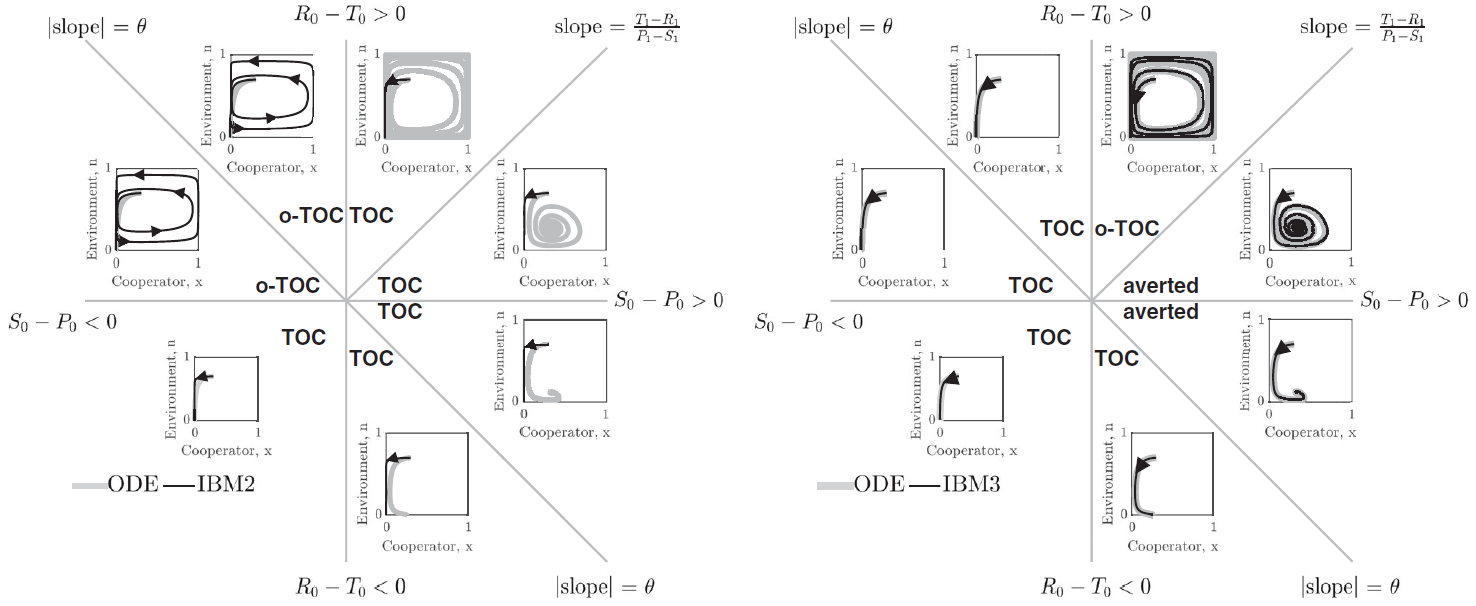
\includegraphics[width=0.9\textwidth]{pictures/Coevolutionary}
% 	\caption{基于IBM动态与复制器模拟的策略与资源协同进化动态。}
% \end{figure}

% 定义扩散系数$D_n$控制相对于人口动态的资源再分配。所有情况都表现出了合作者之间的空间聚集,而在异质环境动态下($D_n=0, D_n=1$),合作者与环境资源状态间也呈现了空间聚集效应。
% \begin{figure}
% 	\label{conevol}
% 	\centering
% 	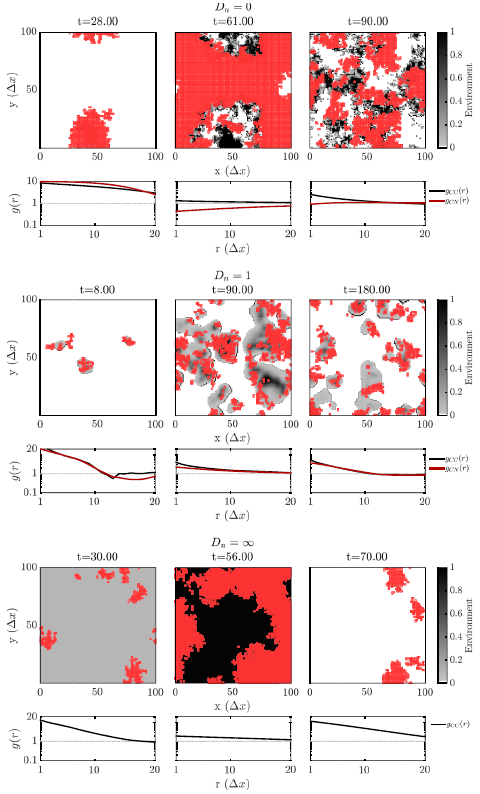
\includegraphics[width=0.9\textwidth]{pictures/D_N}
% 	\caption{资源与合作者的时空动态变化。背景色表示环境,红色正方形表示合作者占据的格子位置,空位被利己者占据。(顶行)$D_n=0$,合作种群的圆波向外扩散;(中排)$D_n=1$,一些小块中的合作者四处移动并分裂;(下排)$D_n=\infty$,大的合作者群体随着时间的推移而扩展和收缩,幅度逐渐增大直到全部消亡。}
% \end{figure}

% 这一模型可进一步用来研究城市共存问题。城市是具有聚集效应的实体,它的复杂性在于它不仅是各个组分的总和,更是各个组分交互作用的产物。以城市产业格局为研究对象,则代价为动态的交易收入或支出,资源可以定义为均匀分布的人口和依赖于距离分布的企业,可结合前述思想预测在城市空间内新企业的产生。思路如下:1)收集公司经济状况及交互距离衰减情况,建立各交易的输入-输出流及当前交互矩阵;2)依赖不同的交易将公司要素进行向量化;3)建立$kN\times kN$的动态矩阵,新公司可能在有利于城市整体发展的最佳地点出现;4)在足够长的时间尺度下模拟这一过程;5)评估模拟得到的产业格局下交易的多样性和产业空间结构的适宜性。一些城市产业结构可能会导致TOC困境,即企业更追求自身利益而忽略城市整体发展。由于城市特性与多样性存在,初始状态会影响城市多样的分化。这一模拟可以帮助我们理解新兴公司在空间和规模上的分布规律。
\chapter{总结与展望}

城市中微元的扩散规律可能会对城市形态和城市要素分布产生很大的影响。所以在此我们额外总结一下人类移动性的模式。通常我们会认为人类的行动是一个连续时间的随机游走(continuous time random walk,即CTRW),与此相关的是数学模型是扩散过程(diffusion limit models)。扩散过程的一个问题是难以解释人类移动的厚尾情形,即现代社会中跨城市尺度的移动。基于此,Mandelbrot提出了列维飞行的概念\cite{doi:10.1142/S0218127408021877}来解释人类移动性的厚尾分布。这两种方式有一个共同的优点,即可以通过随机微分方程的方式得到很多有趣的结论。这两类问题的常用工具Fokker–Planck方程在物理中的意义是粒子在势能场中受到随机力后,随时间演化的位置或是速度的分布函数。这对于我们探究人类移动性对于偶发事件的反应也是有很大帮助的。Chaoming Song于2010年提出的一种双机制模型\cite{song2010modelling}是笔者看到的解释力比较强的人类移动性模型。该模型假设了一种双机制运行,一种长距离跳和短距离扩散由一个概率控制,交替着进行。与该模型相关的有很多类似的概念。比如Watts的小世界网络模型\cite{watts1998collective},依赖的也是长程重连机制。空间社交网络模型\cite{PhysRevX.4.011008}认为,我们每个人的社交网络的更新速度、模式是非常不同的,这依赖于我们与这些“第二邻居”(即朋友的朋友)是怎么建立联系的。这在数学上同样建立在长距离的连接服从幂律分布的前提之上。

近年来,相关研究仍在继续。统计规律在新的数据集上并不成立,使得人们对已有模型的动力学机制产生了怀疑。一些研究\cite{GallottiA}表明,列维飞行无法解释私家车轨迹数据集上体现出的行进时间和速度的行为。人类移动的模式仍然不能被完全理解。但我们可以说,虽然我们仍然对此不解,但却已经是在更高的层次上不解了。人类移动的扩散效应建模的假设里,人的大小是忽略不计的。在进一步研究中,我认为可以将爱因斯坦关系\cite{doi:10.1002/andp.18551700105}融入移动性建模之中,即考虑社会经济条件对人产生的\emph{粘性}。此时在低雷诺数的极限下,迁移率是阻力系数的倒数。我们即可以根据城市的社会经济条件定义城市吸引力(可以由Zipf定律给出近似关系),以统一人类移动性在不同城市间的差异性。其中,随机时间点上的的加速而引起的速度变化。将该机制与行程时间的指数衰减结合起来,会导致出行距离的短尾分布,这可能被误解为带截断的幂律分布。这些结果说明了纯描述性模型的局限性,并提供了移动性的机制解释。

城市体系作为一个研究对象可能会面临一些问题:城市的定义更像是一种聚集的趋势,而不是一种明确的边界。我们尚不清楚大城市是否只是小城市的放大版本,这使人们对将不同规模和历史的不同城市系统混合使用的措施产生了疑问\cite{Depersin2317}。系统科学中,如何圈定一个系统的范围,总是一个核心的问题。对城市范围建模的时候要严格考虑物理背景。比如研究城市化率非常高的国家,比如日本时,我们就不应该用生成模型,而是应该用转移模型来处理。因为新人口加入某个城市的原因不再是出生和从农村进入邻近城市,而是去最合适的城市选择最合适的工作。由于KR模型中,增加新结点连接的边数会增加贫富差距,我们在投入一个新区域的建设的时候,必然要给其足够的初始规模。否则该新城市的人口反而会因为吸引力和持续发展能力不够而被淘汰。简单模型中还有很多平凡的机制,可以导出比较先进,而易理解而不平凡的结论,有待我们进一步发掘。

城市作为越来越多的人的居住环境,其发展规律与性质还不算被完全理解。考虑到城市生态系统的开放性和变动性,公共资源的配置依然是一个困难的问题。我们有必要担心这种困境没有技术上的解决方案。也就是说,没有只需要改变自然科学的技术,而对人类价值观或道德观念几乎不需要或根本不需要改变的解决方案\cite{hardin1968tragedy}。这通常被称为公共地悲剧。但在我看来,公共地悲剧更多是决定论者和空想社会主义者的悲剧。由于空间纵深和时间缓冲的存在,通过合理规划和建模是可以规避个体竞争带来的损害,而给社会以总体收益的。

演化稳定策略\cite{PhysRevE.64.051905}是人口与社会自然选择问题\cite{holt1981the}的解决思路。虽然根据本文第四章的讨论,我们发现城市发展过程中可能会达到的稳态不只有一个,即城市最后的平衡产业结构会有一定的随机性。但每种稳定结构关联的社会关注点是有着丰富的研究背景的。比如重工业城市的空气污染和噪音问题等。如何实现达到稳态后的产业优化则是我们需要努力解决的问题。


\bibliographystyle{plain}
\bibliography{references.bib}
\end{document}
